\chapter{Reading the Paper I: The Question, the Data and the Protocol}\label{ch:paper-setup}

\begin{chapterintro}
You now have every tool the paper uses: complex numbers and series, Fourier analysis, linear algebra and eigenvalues, quantum mechanics on a line, the zeta function and its explicit formula, level statistics, finite differences, fitting, and the statistics of generalization. This chapter begins Part VI, where we stop learning new mathematics and read the paper \cite{soniR1} itself. We read it the way a careful referee would. For each claim we ask what it says in plain words, which earlier chapters supply the tools, what computation stands behind it (and we rerun that computation at small scale with \texttt{qmnt} wherever we can), and how strong it is and where it stops.

This first reading covers the front half of the paper: the abstract, the introduction with its scope statement and its account of prior work (Sec.~I and I~A), the data and the unfolding (Sec.~II~A), the background potential and the solver (Sec.~II~B), the fitting and out-of-sample protocol (Sec.~II~C), the arithmetic oracle and its fitted controls (Sec.~II~D), the disclosure of artificial-intelligence use (Sec.~II~F), Figs.~1 and~2, and steps 1--8 of the reconstruction record in Appendix~A. No result tables are interpreted here in depth; that is the job of Chapters~\ref{ch:paper-memorization}, \ref{ch:paper-arithmetic} and~\ref{ch:paper-spurious-floor}. What this chapter gives you is the protocol: exactly what is computed, against what baseline, and why the baseline is fair.

Where this shows up in the paper: everywhere. Every number in Tables~I--V is an rms or a correlation computed by the protocol of Secs.~II~A--D, and every one of them is judged against the null model defined there.
\end{chapterintro}

\begin{prerequisites}
\item Chapter~\ref{ch:intro}: memorizing versus predicting, training versus held-out data.
\item Chapters~\ref{ch:complex}--\ref{ch:asymptotics}: complex exponentials, Taylor series, Lambert $W$, Brent's method, floating-point precision.
\item Chapters~\ref{ch:fourier-series} and~\ref{ch:fourier-transform}: almost-periodic sums, Fourier resolution, phase-randomized surrogates.
\item Chapters~\ref{ch:linear-algebra}--\ref{ch:least-squares}: vectors and norms, eigenvalues, least squares and ridge.
\item Chapters~\ref{ch:schrodinger}--\ref{ch:perturbation}: $H=-d^2/dx^2+V$ in units $\hbar=2m=1$, bound states in a box, WKB turning points, first-order sensitivity.
\item Chapters~\ref{ch:primes}--\ref{ch:explicit-formula}: primes, the zeta function, $N(T)$, $\Nsm$, smooth zeros, the truncated explicit formula.
\item Chapters~\ref{ch:probability}--\ref{ch:wu-sprung}: rms, Pearson correlation, the Cauchy--Schwarz inequality, GUE statistics, the Hilbert--P\'olya conjecture, the Wu--Sprung potential.
\item Chapters~\ref{ch:finite-differences}--\ref{ch:sparse-frequency}: finite-difference dispersion, Richardson extrapolation, Levenberg--Marquardt fitting, null models, splits, surrogates, sparse frequency search.
\item First-year physics: potential energy curves and turning points, standing waves.
\end{prerequisites}

\section{How to read a research paper}\label{sec:paper-setup-reading}

A textbook proves things and then moves on. A research paper does something different: it makes \emph{claims} and offers \emph{evidence}, and the evidence is usually a computation that you were not present for. Reading such a paper well means keeping the claim and the evidence apart in your head, and checking that the second actually supports the first.

In this part of the book every claim gets the same four questions.
\begin{enumerate}
\item[(a)] \textbf{What does it say?} Restate the claim in plain words, without the technical vocabulary.
\item[(b)] \textbf{Which tools?} Name the chapters of this book that supply the mathematics.
\item[(c)] \textbf{What computation?} Identify the calculation behind the claim and, where it is cheap, rerun a small version yourself.
\item[(d)] \textbf{How strong, and where does it stop?} Is the statement a theorem, a numerical observation, a heuristic explanation, or an open question? Over what range of models and data was it tested?
\end{enumerate}

Question (d) uses the status vocabulary you have met throughout the book: \emph{theorem (proved)}, \emph{proved but beyond this book}, \emph{heuristic or approximate}, \emph{conjecture or open}, and \emph{numerical observation}. Almost everything in the paper is a numerical observation about a specific, scoped family of models. Two background statements are open conjectures: the Riemann hypothesis (RH) and the Hilbert--P\'olya conjecture. The paper never asserts either, and neither will we.

One more piece of reading discipline: the paper reuses some letters. Keep these in mind.
\begin{itemize}
\item $N$ is the number of interior grid points of the finite-difference solver (Sec.~II~B) \emph{and} the counting function $N(T)$ of the zeros (Chapter~\ref{ch:counting-zeros}).
\item $A$ is the first-order sensitivity matrix $A_{nk}$ (Sec.~II~C) \emph{and} the non-Hermitian operator in $H+iA$ (Sec.~II~E).
\item $T$ is the length of a training window in $t$ (Sec.~II~D), \emph{and} the second-order tensors $T^{(n)}$ (Sec.~II~E), \emph{and} the Chebyshev polynomials $T_k$ (Sec.~II~C, ``Other bases'').
\end{itemize}
Context always tells you which is meant, but only if you are watching for it.

\begin{keyideas}
\item Separate claim from evidence; for each claim ask (a) what, (b) which tools, (c) which computation, (d) how strong and how far.
\item Nearly every result in the paper is a scoped numerical observation; RH and Hilbert--P\'olya are open conjectures.
\item The symbols $N$, $A$ and $T$ each carry more than one meaning in the paper.
\end{keyideas}

\section{The abstract, sentence by sentence}\label{sec:paper-setup-abstract}

An abstract compresses a whole paper into a paragraph, so every word is load-bearing. The paper's abstract has eight sentences; we take them one at a time. \Cref{tab:paper-setup-abstract} collects where each is substantiated.

\paragraph{S1.} ``Empirical Hilbert--P\'olya constructions fit quantum Hamiltonians to the nontrivial Riemann zeros and judge success by the quality of the fit.''

(a) There is a line of work that builds a quantum system whose energy levels are supposed to match the heights $t_n$ of the zeta zeros, and those works have measured success by how well the levels match the zeros used to build the system. (b) Chapters~\ref{ch:hilbert-polya} and~\ref{ch:wu-sprung}. (c) No computation; this is a description of the literature, supported in Sec.~I~A and by the audit in Appendix~A. (d) It is a characterization of prior work. Its strength rests on the literature audit, whose limits we examine in \cref{sec:paper-setup-prior}.

\paragraph{S2.} ``We apply the test this program has lacked: out-of-sample prediction.''

(a) The paper hides some zeros from the fitting procedure and asks whether the fitted system predicts them. (b) Chapter~\ref{ch:generalization}. (c) The protocol of Sec.~II~C. (d) ``Has lacked'' is again a claim about the literature, hedged in the body as ``to our knowledge''.

\paragraph{S3.} ``Fluctuation potentials on the Wu--Sprung background with up to 900 fitted coefficients, in cosine, Chebyshev, and local piecewise-linear bases, fit their training zeros closely yet show no reproducible held-out predictive skill relative to the unfitted potential, whether the held-out zeros lie above the training range or are interleaved with it.''

(a) Take the smooth Wu--Sprung potential, add a correction built from up to 900 adjustable numbers, tune them so the levels match the training zeros. The match is good, but the tuned system predicts hidden zeros no better than the untuned one, whether the hidden zeros are higher up or mixed in among the training ones. (b) Chapters~\ref{ch:wu-sprung}, \ref{ch:finite-differences}, \ref{ch:fitting}, \ref{ch:generalization}. (c) Tables~I--III (paper Sec.~III), analysed in Chapter~\ref{ch:paper-memorization}. (d) Note the qualifiers. ``Wu--Sprung background'': one background potential. ``Cosine, Chebyshev, and local piecewise-linear'': three bases. ``Reproducible'': one Chebyshev row is marginal (Table~II), and the paper says so. ``Relative to the unfitted potential'': the comparison is with a specific null, which we define in \cref{sec:paper-setup-nulls}.

\paragraph{S4.} ``They fit shuffled and phase-randomized surrogate targets as well as the real zeros and, trained on a pure prime-2 explicit-formula oscillation, fail to continue it beyond the training window.''

(a) Two diagnostic experiments. First, scramble the target fluctuations (by shuffling, or by keeping the power spectrum and randomizing phases) and refit: the fit is just as good, so fit quality does not detect real structure. Second, replace the target by a single known periodic-looking signal, the $p=2$ term of the explicit formula (our running example RE2), and ask whether the fitted potential keeps oscillating past the training window: it does not. (b) Chapters~\ref{ch:fourier-transform}, \ref{ch:controls}, \ref{ch:explicit-formula}. (c) Paper Sec.~III, paragraphs ``Permutation and surrogate tests'' and ``Arithmetic-continuation probe''. (d) Numerical observations on the scale-1, $M=400$ configuration; Chapter~\ref{ch:paper-memorization} gives the numbers.

\paragraph{S5.} ``By contrast, a truncation of the Riemann--von Mangoldt explicit formula with zero fitted parameters predicts held-out zeros with correlation up to $+0.99$ through zero $10^4$.''

(a) A formula built from a handful of primes, with nothing tuned to the zeros at all, predicts the hidden zeros well, and keeps doing so up to the ten-thousandth zero. (b) Chapter~\ref{ch:explicit-formula}. (c) Table~V; we reproduce two of its entries in \cref{sec:paper-setup-oracle}. (d) Numerical observation. The formula is classical and the paper claims no novelty for it (Sec.~I~A~b).

\paragraph{S6.} ``Controls with fitted sinusoidal models show that the obstacle is the parametrization, not the parameter count: a dense 900-coefficient Fourier model also stays near the null, while a fitted control given only a sparsity prior in frequency, and no arithmetic input, recovers frequencies at $\log p^m$ from 400 zeros and predicts held-out zeros with correlation $+0.99$.''

(a) Two more fitted models, neither told about primes. One has 900 coefficients spread over a uniform grid of frequencies and stays within 0.005 of the null. The other is told only ``the signal is a sum of a few sinusoids'', finds the frequencies by search, and those frequencies turn out to sit at logarithms of prime powers; it predicts as well as the 25-prime formula. So the number of parameters is not what matters; their form is. (b) Chapters~\ref{ch:fourier-transform}, \ref{ch:least-squares}, \ref{ch:sparse-frequency}. (c) Table~IV, Sec.~IV; Chapter~\ref{ch:paper-arithmetic}. (d) Numerical observation. The paper itself calls ``sparse in $t$-frequency'' ``a strong and well-chosen prior'' and notes the concentration of the zeros' spectrum at $\log p^m$ is classical \cite{landau,gonek}.

\paragraph{S7.} ``A subsidiary dissection of second-order non-Hermitian perturbations shows how surrogate optimization outside its validity range can manufacture an apparently meaningful in-sample floor; exact diagonalization dissolves it.''

(a) A side study: a different model family, fitted through a perturbative approximation, appeared to hit a common error floor; checking the exact spectrum showed the floor was an artifact. (b) Chapters~\ref{ch:perturbation} and~\ref{ch:non-hermitian}. (c) Sec.~V, Fig.~5; Chapter~\ref{ch:paper-spurious-floor}. (d) Labelled ``subsidiary''; Sec.~VI states it was not rerun for the revision.

\paragraph{S8.} ``We propose held-out prediction as a minimal falsifiability standard for empirical operator claims and provide the protocol, baselines, and a complete reconstruction record.''

(a) A recommendation for future work, plus the materials to check this work. (b) Chapters~\ref{ch:generalization} and~\ref{ch:controls}. (c) Sec.~VI items (i)--(iv); Appendix~A; the Zenodo record \cite{zenodo}. (d) A proposal, not a result; Chapter~\ref{ch:paper-critique} discusses it.

\begin{table}[htbp]\centering
\caption{Where each sentence of the abstract is substantiated in the paper (R1 numbering) and which chapter of this book reads it.}\label{tab:paper-setup-abstract}
\small
\begin{tabular}{p{0.07\linewidth}p{0.36\linewidth}p{0.24\linewidth}p{0.2\linewidth}}
\toprule
sentence & content & paper location & read in \\
\midrule
S1 & prior work judged by fit quality & Sec.~I, I~A, App.~A audit & this chapter \\
S2 & the out-of-sample test & Sec.~II~C & this chapter \\
S3 & fits memorize, do not predict & Sec.~III, Tables I--III, Fig.~3 & Ch.~\ref{ch:paper-memorization} \\
S4 & surrogates and continuation probe & Sec.~III & Ch.~\ref{ch:paper-memorization} \\
S5 & explicit formula predicts & Sec.~IV, Table~V, Fig.~1 & this chapter, Ch.~\ref{ch:paper-arithmetic} \\
S6 & fitted sinusoidal controls & Sec.~II~D, IV, Table~IV & Ch.~\ref{ch:paper-arithmetic} \\
S7 & spurious non-Hermitian floor & Sec.~II~E, V, Fig.~5 & Ch.~\ref{ch:paper-spurious-floor} \\
S8 & falsifiability standard, record & Sec.~VI, App.~A & Ch.~\ref{ch:paper-critique} \\
\bottomrule
\end{tabular}
\end{table}

\begin{checkpoint}
Which sentence of the abstract would become false if the sparse-frequency control C2 had selected frequencies unrelated to prime powers, and which sentences would be unaffected?
\end{checkpoint}
\checkanswer{S6 would lose its second half (``recovers frequencies at $\log p^m$''). S1--S5, S7 and S8 do not mention C2 and would be unaffected; in particular S3 and S5 concern the fitted potentials and the oracle, which do not involve C2.}

\begin{keyideas}
\item The abstract makes three kinds of statement: about prior work (S1, S2), about numerical results (S3--S7), and a methodological proposal (S8).
\item Every result sentence carries scope qualifiers (one background, three bases, ``reproducible'', ``relative to the unfitted potential''); keep them when you summarize.
\end{keyideas}

\section{The question and its scope}\label{sec:paper-setup-question}

\subsection{The Hilbert--P\'olya motivation}

The paper's first sentence states the Hilbert--P\'olya conjecture: the heights $t_n$ of the nontrivial zeros $\rho_n=\tfrac12+it_n$ of $\zeta(s)$ are the spectrum of a self-adjoint operator. Recall from Chapter~\ref{ch:eigen} that a self-adjoint (Hermitian) operator has real eigenvalues; if the $t_n$ were such eigenvalues they would be real, which is the statement that every nontrivial zero lies on the critical line. That is why the conjecture, if realized by a concrete operator, would prove RH (Chapter~\ref{ch:hilbert-polya}). The conjecture is open. The notation $\rho_n=\tfrac12+it_n$ presumes the zeros used are on the critical line, which is numerically verified for every zero the paper uses; it presumes nothing about zeros in general.

The paper lists three pieces of ``circumstantial evidence'' with their sources.
\begin{enumerate}
\item Montgomery's pair-correlation theorem and Odlyzko's numerics match GUE eigenvalue statistics \cite{montgomery,odlyzko87}. Status: Montgomery's result is a theorem proved under the assumption of RH, and only for test functions whose Fourier transform vanishes outside the interval $(-1,1)$ (this is the restriction on the test functions; compare the statement of Montgomery's pair correlation in Chapter~\ref{ch:level-statistics}); the full pair-correlation statement, without that restriction, is a conjecture; Odlyzko's agreement is a numerical observation (Chapter~\ref{ch:level-statistics}).
\item The zero-counting function resembles a semiclassical trace formula in which primes play the role of periodic orbits \cite{berrykeating99,schumayer}. Status: an analogy (Chapter~\ref{ch:hilbert-polya}).
\item Explicit operator candidates continue to be proposed \cite{connes,bbm,bellissard,sierra,recenthp1,recenthp2,zetatriples}. Status: no proposal is accepted as an operator whose spectrum is the zeros (Chapter~\ref{ch:hilbert-polya}).
\end{enumerate}
None of this is evidence that any particular operator exists, and the paper does not say it is.

\subsection{The empirical program and its implicit logic}

The second paragraph of Sec.~I introduces the target. Wu and Sprung \cite{wusprung} built a smooth one-dimensional potential from the average density of zeros (Chapter~\ref{ch:wu-sprung}) and added fitted corrections to reproduce the low zeros; successors refined this \cite{vanzyl,slater,jaksch}. The paper names the reasoning that such work implicitly relies on:

\begin{quote}
``The implicit logic is that a potential reproducing many zeros accurately has captured something about the putative zeta operator.''
\end{quote}

The paper tests this logic by the standard you met in Chapter~\ref{ch:generalization}: a model fitted to zeros $1,\dots,n_{\rm fit}$ ``has captured structure, rather than data, only to the extent that it predicts zeros it was not shown.'' Remember the student who memorizes last year's exam answers (Chapter~\ref{ch:intro}). Reproducing those answers perfectly says nothing about this year's exam. The fit quality on training zeros is the analogue of reproducing last year's answers.

\subsection{The scope statement}

Immediately after naming the test, the paper limits its own claim. Read this paragraph slowly, because every later claim inherits it. What is tested:
\begin{itemize}
\item only empirical inverse-spectral constructions whose parameters are fitted to finite sets of zeros;
\item among those, only fluctuation potentials added to the Wu--Sprung background;
\item in three bases (cosine, Chebyshev, hat; Sec.~II~C).
\end{itemize}
What is explicitly not tested:
\begin{itemize}
\item other backgrounds;
\item other parametrizations: Hermite functions, wavelets, neural-network potentials;
\item analytic Hilbert--P\'olya constructions, ``in which an operator is specified independently of the zeros and its spectrum is then predicted''. The paper makes ``no claim against'' these.
\end{itemize}
Two definitions close the paragraph. First, ``capture'' is operational: ``predictive transfer to held-out zeros, measured by rms error and correlation relative to the model's own smooth baseline.'' Second, the novelty claimed is ``not the explicit formula or any representation of the zeros, but the controlled out-of-sample comparison and the associated falsifiability protocol.''

The operational definition of ``capture'' is worth dwelling on. It replaces a vague word (has the model ``captured'' the zeta operator?) with two measurable numbers (rms error and correlation on hidden zeros) compared with a third (the same numbers for the model's own smooth part). We define all three precisely in \cref{sec:paper-setup-protocol,sec:paper-setup-nulls}.

\begin{pitfall}
Do not read the paper as saying ``no potential can encode the Riemann zeros'' or ``the Hilbert--P\'olya conjecture is false''. Its claim concerns fitted fluctuation potentials on one background, in three bases, under one fitting protocol. Sec.~VI is explicit: ``This is evidence about the tested parametrizations and optimizer together, not a statement about what a potential can represent.''
\end{pitfall}

\subsection{The headline result and Fig.~1}

The third paragraph of Sec.~I summarizes the outcome. Smooth potentials with a few hundred basis coefficients reproduce any prefix of the zeros to machine-level accuracy in-sample, yet their out-of-sample predictions show no reproducible correlation with the truth across all the scales, splits, bases, budgets, regularization settings and restarts examined. A formula with zero fitted parameters, the explicit formula truncated to a handful of primes, predicts held-out zeros with high and nearly height-independent skill through zero $10^4$. The paragraph ends with a hedge you should keep: ``within the operator families tested, the fits do not recover it, although a model with a non-arithmetic sparsity prior does.''

Paper Fig.~1 is the whole story in one picture. Zeros 370--460 are shown; the fit used zeros 1--400 at scale~1 with $M=400$ cosine coefficients. Inside the training region both curves track the true fluctuation. Past index 400 the fitted operator's prediction has held-out correlation $-0.07$, while the six-prime explicit formula has $+0.96$ (both numbers from the Fig.~1 caption). Neither curve uses any zero past the boundary. We reproduce the oracle half of this figure in \cref{sec:paper-setup-oracle} (\cref{fig:paper-setup-oracle}); the operator half requires a full potential fit, which Chapter~\ref{ch:paper-memorization} discusses.

\begin{checkpoint}
The scope statement says the paper makes no claim against analytic Hilbert--P\'olya constructions. In one sentence, why would an out-of-sample test not even apply to such a construction?
\end{checkpoint}
\checkanswer{An analytic construction is specified without fitting to any zeros, so every zero is already ``held out''; there is no training set whose memorization could masquerade as prediction.}

\begin{keyideas}
\item The question: does a potential fitted to zeros $1,\dots,n_{\rm fit}$ predict zeros it was not shown?
\item The scope: Wu--Sprung background, three bases, fitted parameters; analytic constructions are not targeted.
\item ``Capture'' means held-out rms and correlation compared with the model's own smooth baseline.
\item The paper claims novelty only for the controlled comparison and protocol.
\end{keyideas}

\section{Four strands of prior work and the literature audit}\label{sec:paper-setup-prior}
% DYK-BEGIN
\begin{didyouknow}{Stigler's Law}
In 1980 the statistician Stephen Stigler proposed that no scientific discovery is named after its original discoverer, and he jokingly credited this law to the sociologist Robert Merton. This book has examples: the Gaussian curve appeared in de Moivre's work, and Gauss used the FFT long before Cooley and Tukey. A good literature audit checks who really did what first.
\end{didyouknow}
% DYK-END

Sec.~I~A places the work among four strands of literature. \Cref{tab:paper-setup-strands} summarizes them by three yes/no questions.

\paragraph{(a) Inverse-spectral fits to the zeros.} Wu and Sprung \cite{wusprung} inverted the smooth counting function into a semiclassical potential and added fitted corrections; van Zyl and Hutchinson \cite{vanzyl} and Slater \cite{slater} extended the fractal fits; Jaksch \cite{jaksch} generated successive zeros from a Wu--Sprung-type potential and traced the fractal corrections to the Riemann--von Mangoldt approximation error; Schumayer and Hutchinson \cite{schumayer} review the tradition. The paper's claim: these models ``have been evaluated primarily by agreement with the zeros used in their construction; to our knowledge, no systematic held-out test of predictive performance has been reported in this literature''.

\paragraph{(b) Explicit formulae for the $n$-th zero.} Fran\c{c}a and LeClair \cite{francaleclair,leclair} derived a transcendental equation for the $n$-th zero whose smooth part is the Lambert-$W$ asymptotic of the counting function (we derive this smooth part in \cref{sec:paper-setup-data}), and developed it with prime corrections. These are truncations of the classical Riemann--von Mangoldt/Guinand--Weil explicit formula (Chapter~\ref{ch:explicit-formula}). The paper uses such a truncation as an ``information-existence baseline'' and claims no novelty for it. It also cites Connes \cite{connes26}: extremizing a truncated Weil quadratic form over primes $p\le13$ yields approximations to the first 50 zeros with accuracies from $10^{-3}$ down to $2.6\times10^{-55}$, provably on the critical line. The paper places this on the arithmetic side of its comparison (it uses prime data only and fits nothing to zeros) and says its existence strengthens the conclusion that the predictive information is arithmetic.

\paragraph{(c) Machine learning on zeta zeros and arithmetic data.} Direct regression of zero positions by generic machine-learning models has been explored \cite{sdsu} ``in an interpolation setting without operator structure''. He, Lee, Oliver and collaborators have machine-learned number-theoretic structures \cite{henumberfields,vanishingorder}, and the murmurations of elliptic-curve $L$-functions were discovered through machine-learning-driven exploration \cite{murmurations}. The paper's contrast: that literature asks what is learnable from arithmetic data; this paper asks what a physically structured model family fails to learn from spectral data.

\paragraph{(d) Operator proposals.} The analytic program \cite{berrykeating99,connes,bbm,sierra,recenthp1,recenthp2,zetatriples} seeks exact operators and ``is not our target''. The zeta spectral triples of Connes, Consani and Moscovici \cite{zetatriples} build operators from Euler products over primes, with numerically observed spectral convergence; like \cite{connes26} this is prime-driven, not a fit to zero data.

\begin{table}[htbp]\centering
\caption{The four strands of prior work in paper Sec.~I~A, classified by the paper's own description. ``Fitted to zeros'' means parameters are adjusted to match computed zeros.}\label{tab:paper-setup-strands}
\small
\begin{tabular}{p{0.3\linewidth}p{0.14\linewidth}p{0.18\linewidth}p{0.22\linewidth}}
\toprule
strand & operator? & fitted to zeros? & held-out test reported? \\
\midrule
(a) inverse-spectral fits & yes & yes & none found \\
(b) explicit formulae & no & no & not applicable \\
(c) machine learning & no & yes for zero regression \cite{sdsu}; others fit arithmetic data & yes (train/test splits) \\
(d) operator proposals & yes & no & not applicable \\
\bottomrule
\end{tabular}
\end{table}

The sentence that sums up the positioning: ``ML papers that predict zero sequences use train/test splits but involve no operator; inverse-spectral papers have operators but no held-out evaluation; we found the intersection empty.'' The paper's own work is the combination missing from \cref{tab:paper-setup-strands}: operator yes, fitted to zeros yes, held-out test yes.

\subsection{The literature audit: basis and limits}

How does the paper support ``no systematic held-out test \dots has been reported''? Appendix~A records a citation-graph audit: among all works citing Wu--Sprung \cite{wusprung} and van Zyl--Hutchinson \cite{vanzyl} indexed by Semantic Scholar (accessed August 2026; 28 and 29 works respectively), none mentions prediction, generalization, held-out evaluation, or machine learning; Slater \cite{slater} and Jaksch \cite{jaksch} had no indexed citations.

Apply question (d). The audit is reproducible, which is a real strength: anyone can rerun the same query. But it is bounded in four ways.
\begin{enumerate}
\item \textbf{Coverage of the graph.} Only works that cite \cite{wusprung} or \cite{vanzyl} are examined. A paper that fitted a potential to zeros and tested it on held-out zeros without citing either would be missed.
\item \textbf{Coverage of the index.} Only works indexed by one database at one date are examined.
\item \textbf{Keyword method.} The test is whether the listed words are mentioned. A held-out test described in other words (for example ``extrapolation to higher zeros'') could be missed; a mention of ``prediction'' in an unrelated sense would count as a mention.
\item \textbf{Absence versus nonexistence.} The audit shows that nothing was found inside a bounded search, not that nothing exists.
\end{enumerate}
The paper's wording respects these limits: ``to our knowledge'' and ``we found the intersection empty''. When you summarize this part of the paper, keep both phrases. Chapter~\ref{ch:paper-critique} lists the audit among the points a referee could press.

\begin{checkpoint}
Suppose a 2015 paper fitted a potential to zeros $1$--$100$ and reported its error on zeros $101$--$120$, but cited only Berry and Keating. Would the paper's audit find it?
\end{checkpoint}
\checkanswer{No. The audit examines only works citing \cite{wusprung} or \cite{vanzyl}, so a work citing neither is outside the searched set, however relevant it is.}

\begin{keyideas}
\item Four strands: inverse-spectral fits (operator, fitted, no held-out test found), explicit formulae (arithmetic, nothing fitted), machine learning (fitted, held-out, no operator), operator proposals (operator, nothing fitted).
\item The novelty claim rests on a reproducible but bounded citation-graph keyword audit; the paper hedges it with ``to our knowledge''.
\item Prime-only constructions such as \cite{connes26} sit on the arithmetic side of the comparison.
\end{keyideas}

\section{The data: zeros, smooth zeros and fluctuations}\label{sec:paper-setup-data}

\subsection{The zeros and their precision}

Sec.~II~A and Appendix~A step~1: zeros $t_1,\dots,t_{1000}$ were computed with \texttt{mpmath.zetazero(n)} at 20 significant digits, with $t_1=14.134725141734695$ and $t_{1000}=1419.42248094599$; zeros $10^3$--$10^4$ at 15 digits. The paper asserts that ``both precisions exceed every use below by many orders''. You quantify this in Problem~25: the smallest held-out error the paper reports is about 0.02 mean spacings (Table~IV), and its tightest in-sample statement is rms $<10^{-4}$ spacings (Sec.~III), while 15 significant digits at height $10^4$ fix a zero to roughly $10^{-11}$ in $t$, at least seven orders of magnitude below either.

\subsection{The smooth counting function and the mean spacing}

Recall from Chapter~\ref{ch:counting-zeros} that $N(T)$ counts zeros with $0<t\le T$, and that the Riemann--von Mangoldt formula splits it into a smooth part plus a small oscillating remainder $S(T)$. The paper's Eq.~(1) is the smooth part,
\begin{equation}
\Nsm(t)=\frac{t}{2\pi}\log\frac{t}{2\pi}-\frac{t}{2\pi}+\frac78 ,
\label{eq:paper-setup-nsm}
\end{equation}
with $\log$ the natural logarithm. Its derivative will give the mean spacing, so let us compute it line by line.
\begin{align}
\frac{d\Nsm}{dt}&=\frac{d}{dt}\Bigl[\frac{t}{2\pi}\log\frac{t}{2\pi}\Bigr]-\frac{1}{2\pi}
&&\text{(the constant $\tfrac78$ has zero derivative)}\nonumber\\
&=\frac{1}{2\pi}\log\frac{t}{2\pi}+\frac{t}{2\pi}\cdot\frac{1}{t}-\frac{1}{2\pi}
&&\text{(product rule; $\tfrac{d}{dt}\log\tfrac{t}{2\pi}=\tfrac1t$)}\nonumber\\
&=\frac{1}{2\pi}\log\frac{t}{2\pi}. \label{eq:paper-setup-dnsm}
\end{align}
Differentiating once more,
\begin{equation}
\frac{d^2\Nsm}{dt^2}=\frac{1}{2\pi t}.
\label{eq:paper-setup-d2nsm}
\end{equation}
For $t>2\pi$ the derivative \eqref{eq:paper-setup-dnsm} is positive, so $\Nsm$ is increasing there and can be inverted.

The \emph{smooth zeros} $s_n$ are defined (Sec.~II~A) by
\begin{equation}
\Nsm(s_n)=n-\tfrac12 .
\label{eq:paper-setup-sn}
\end{equation}
The half reflects the convention (Chapter~\ref{ch:counting-zeros}) that $N(t)$ jumps from $n-1$ to $n$ at $t_n$, so its midpoint value there is $n-\tfrac12$. Treat $n$ as a continuous variable and differentiate \eqref{eq:paper-setup-sn} with respect to $n$ using the chain rule:
\begin{equation}
\Nsm'(s_n)\,\frac{ds_n}{dn}=1
\quad\Longrightarrow\quad
\gap_n\equiv\frac{ds_n}{dn}=\frac{1}{\Nsm'(s_n)}=\frac{2\pi}{\log(s_n/2\pi)} ,
\label{eq:paper-setup-gap}
\end{equation}
where the last step substitutes \eqref{eq:paper-setup-dnsm}. This is the local mean spacing, the paper's $\gap_n$. Appendix~A step~2 computes it numerically as \texttt{np.gradient} of the array of smooth zeros, a centred difference that agrees closely with \eqref{eq:paper-setup-gap} except at the two ends of the array (see the pitfall below).

The \emph{fluctuation} of zero $n$, in units of the local mean spacing, is
\begin{equation}
f_n=\frac{t_n-s_n}{\gap_n}.
\label{eq:paper-setup-fluct}
\end{equation}
This is what every model in the paper tries to predict. ``All errors below are quoted in units of the local mean spacing'' (Sec.~II~A), and Appendix~A adds that this spacing is computed from the smooth zeros of Eq.~(1). Dividing by $\gap_n$ makes errors comparable across heights: near zero 1 the mean spacing is several units of $t$, near zero 1000 it is just over one (see the first and third Sample Problems of this section, below).

\begin{sample}{Unfolding the first zero}
Find $s_1$, $\gap_1$ and the fluctuation $f_1$ of the first zero $t_1=14.134725$ (RE1).

\textbf{Step 1: set up the equation.} By \eqref{eq:paper-setup-sn}, $s_1$ solves $\Nsm(s)=\tfrac12$.

\textbf{Step 2: bracket.} At $t=14$: $t/2\pi=2.22817$, $\log(2.22817)=0.80117$, so $\Nsm(14)=2.22817\times0.80117-2.22817+0.875=0.432$, which is below $\tfrac12$. At $t=15$, $t/2\pi=2.38732$, $\log=0.87018$, $\Nsm(15)=2.07738-2.38732+0.875=0.565$, above $\tfrac12$. The root is in $(14,15)$.

\textbf{Step 3: Newton steps.} With \eqref{eq:paper-setup-dnsm}, $\Nsm'(14)=0.80117/2\pi=0.1275$. Carried to four decimals, $\Nsm(14)=0.4320$, so the first iterate is $s^{(1)}=14+(0.5-0.4320)/0.1275=14+0.533=14.533$. At this point $\Nsm(14.533)=0.5016$ and $\Nsm'(14.533)=0.1335$, so the second iterate is $s^{(2)}=14.533-(0.5016-0.5)/0.1335=14.533-0.0120=14.521$. A third Newton step changes $s$ by less than $10^{-5}$, so $s_1\approx14.521$.

\textbf{Step 4: spacing.} $\gap_1=2\pi/\log(14.521/2\pi)=6.28319/0.83775=7.500$.

\textbf{Step 5: fluctuation.} $f_1=(14.134725-14.521)/7.500=-0.0515$.
\[
\boxed{s_1\approx14.521,\quad \gap_1\approx7.500,\quad f_1\approx-0.052}
\]
The first zero sits about one twentieth of a mean spacing below its smooth position.
\end{sample}

\subsection{The Lambert-$W$ form of the smooth zeros}

Sec.~I~A~b says the smooth part of the Fran\c{c}a--LeClair equation is ``the Lambert-$W$ asymptotic of the counting function''. Recall from Chapter~\ref{ch:asymptotics} that the Lambert function $W(z)$ is defined by $W(z)\,e^{W(z)}=z$; for $-1/e\le z<0$ there are two real values, and the principal branch $W_0$ is the one with $W_0\ge-1$.

\begin{sample}{Solving $\Nsm(s_n)=n-\tfrac12$ in closed form}
Derive a closed form for $s_n$ and evaluate it at $n=1$.

\textbf{Step 1: collect terms.} From \eqref{eq:paper-setup-nsm} and \eqref{eq:paper-setup-sn},
\[
\frac{s}{2\pi}\log\frac{s}{2\pi}-\frac{s}{2\pi}=n-\tfrac12-\tfrac78=n-\tfrac{11}{8},
\qquad\text{so}\qquad
\frac{s}{2\pi}\Bigl(\log\frac{s}{2\pi}-1\Bigr)=n-\tfrac{11}{8}.
\]

\textbf{Step 2: substitute.} Let $u=s/(2\pi e)$. Then $s/2\pi=eu$ and $\log(s/2\pi)-1=\log(eu)-1=\log u$. The equation becomes $eu\log u=n-\tfrac{11}8$, that is
\[
u\log u=z,\qquad z\equiv\frac{n-11/8}{e}.
\]

\textbf{Step 3: recognize $W$.} Put $w=\log u$, so $u=e^w$: then $we^w=z$, hence $w=W(z)$.

\textbf{Step 4: back-substitute.} From $W e^W=z$ we get $e^{W}=z/W$, so $u=e^{W(z)}=z/W(z)$ and
\begin{equation}
s_n=2\pi e\,u=\frac{2\pi e\,z}{W(z)}=\frac{2\pi\,(n-11/8)}{W\!\bigl((n-11/8)/e\bigr)} .
\label{eq:paper-setup-lambert}
\end{equation}

\textbf{Step 5: choose the branch.} For $n\ge2$, $z>0$ and $W$ has one real value. For $n=1$, $z=-0.375/e=-0.13795$, which lies in $(-1/e,0)$, so there are two real branches. The branch $W_{-1}<-1$ gives $u<1/e$, i.e.\ $s<2\pi$, where $\Nsm$ is decreasing and not a counting function. We need $W_0$.

\textbf{Step 6: evaluate.} $W_0(-0.13795)=-0.16225$ (check: $-0.16225\,e^{-0.16225}=-0.16225\times0.85023=-0.13795$). Then $s_1=2\pi(-0.375)/(-0.16225)=14.521$.
\[
\boxed{s_n=\frac{2\pi(n-11/8)}{W_0\bigl((n-11/8)/e\bigr)},\qquad s_1\approx14.521}
\]
This agrees with the Sample Problem ``Unfolding the first zero''. The paper itself solves \eqref{eq:paper-setup-sn} by Brent's method (Appendix~A step~2); both routes give the same $s_n$.
\end{sample}

\begin{sample}{What ``0.263 mean spacings'' means in height}
The paper's null error on zeros 401--500 is 0.2631 spacings (Sec.~II~C; Appendix~A ``Key anchors''). Convert this to units of $t$ near zero 500, and find the mean spacing at zero 1000 too.

\textbf{Step 1: spacing near zero 500.} Use $t_{500}=811.1843588465$ (Appendix~A anchors) in \eqref{eq:paper-setup-gap} as an estimate of $s_{500}$: $811.18/2\pi=129.10$, $\log(129.10)=4.8606$, so the spacing is $2\pi/4.8606=1.293$.

\textbf{Step 2: convert.} $0.263\times1.293=0.340$ units of $t$.

\textbf{Step 3: spacing at zero 1000.} $1419.42/2\pi=225.91$, $\log(225.91)=5.4201$, spacing $=2\pi/5.4201=1.159$.
\[
\boxed{\gap\approx1.293\ \text{near }n=500,\quad 0.263\ \text{spacings}\approx0.340\ \text{in }t,\quad \gap\approx1.159\ \text{near }n=1000}
\]
\end{sample}

\subsection{Fluctuations and the counting residual}

The sinusoidal models of Sec.~II~D are trained not on $f_n$ but on
\begin{equation}
y_n=n-\tfrac12-\Nsm(t_n),
\label{eq:paper-setup-yn}
\end{equation}
the amount by which the smooth count misses the midpoint count at the true zero. These two quantities are nearly negatives of each other. To see it, let $\delta_n=t_n-s_n$ and expand $\Nsm$ about $s_n$ using Taylor's theorem with remainder, which we state here.
\begin{beyond}
Taylor's theorem with the Lagrange remainder: if $g$ has a continuous second derivative on an interval containing $s$ and $s+\delta$, then $g(s+\delta)=g(s)+g'(s)\,\delta+\tfrac12 g''(\xi)\,\delta^2$ for some $\xi$ between $s$ and $s+\delta$. We take it on trust; a proof (by repeated use of the mean value theorem) is in \cite{rhb}.
\end{beyond}
With $g=\Nsm$, $s=s_n$ and $\delta=\delta_n$:
\begin{align}
\Nsm(t_n)&=\Nsm(s_n)+\Nsm'(s_n)\,\delta_n+\tfrac12\Nsm''(\xi_n)\,\delta_n^2
&&\text{($\xi_n$ between $s_n$ and $t_n$)}\nonumber\\
&=n-\tfrac12+\frac{\delta_n}{\gap_n}+\frac{\delta_n^2}{4\pi\xi_n}
&&\text{(by \eqref{eq:paper-setup-sn}, \eqref{eq:paper-setup-gap}, \eqref{eq:paper-setup-d2nsm})}.\nonumber
\end{align}
Substituting into \eqref{eq:paper-setup-yn} and using $f_n=\delta_n/\gap_n$,
\begin{equation}
y_n=-f_n-\frac{\delta_n^2}{4\pi\xi_n}.
\label{eq:paper-setup-ynfn}
\end{equation}
The correction is tiny: at $n=500$, $|y_n+f_n|\approx7\times10^{-6}$; even at $n=1$ it is about $8\times10^{-4}$ (Problem~15). So, to excellent accuracy, the counting residual is minus the fluctuation in spacings. A zero that lies \emph{above} its smooth position ($f_n>0$) is one where the smooth count has \emph{overshot} the midpoint count ($y_n<0$).

\begin{pitfall}
Mind the sign in \eqref{eq:paper-setup-ynfn}. The explicit formula approximates $S(t)$, the excess of the true count over the smooth count (Chapter~\ref{ch:counting-zeros}); at the zeros, $S$ is approximately $y_n$, hence approximately $-f_n$. If you plot $\Nfl(t_n)$ against $f_n$ and see a strong \emph{negative} correlation, you have not made an error.
\end{pitfall}

\begin{pitfall}
\texttt{np.gradient} uses centred differences in the interior of an array and one-sided differences at its ends. At $n=1$ it returns $s_2-s_1\approx6.13$ instead of the analytic $\gap_1\approx7.50$ of \eqref{eq:paper-setup-gap}. This affects only the end points; recomputing the null rms over the window of zeros 1--400 with the spacings returned by \texttt{np.gradient} (one-sided at both ends of that window) changes it by less than $10^{-4}$, far below the precision of any table. (This was checked for that window only.) The lesson is general: know what your library does at the boundary.
\end{pitfall}

\begin{pycode}
import numpy as np, qmnt
from scipy.special import lambertw

def Nsm(t):                      # paper Eq. (1)
    u = t / (2*np.pi)
    return u*np.log(u) - u + 7/8

def smooth_zero(n):              # Lambert-W form, principal branch
    z = (n - 11/8) / np.e
    return 2*np.pi*(n - 11/8) / np.real(lambertw(z, 0))

def gap(s):                      # local mean spacing
    return 2*np.pi / np.log(s / (2*np.pi))

t = qmnt.zeros(1000)             # t_1 ... t_1000
n = np.arange(1, 1001)
s = smooth_zero(n)
f = (t - s) / gap(s)             # fluctuations in mean spacings

for lo, hi in [(1, 400), (401, 500), (801, 1000)]:
    sel = (n >= lo) & (n <= hi)
    print(lo, hi, np.sqrt(np.mean(f[sel]**2)))   # null rms
\end{pycode}

Running this listing prints null values within $0.002$ of the paper's anchor 0.2631 for zeros 401--500, and within $0.004$ of its anchors 0.2438 (zeros 1--400) and 0.2739 (zeros 801--1000) (Appendix~A). (The paper's anchors are measured against the unperturbed potential's levels; \cref{sec:paper-setup-nulls} bounds the difference from the smooth-zero values by 0.063 and discusses why it is in practice much smaller. That the values agree as closely as they do is a numerical observation.)

\begin{figure}[htbp]\centering
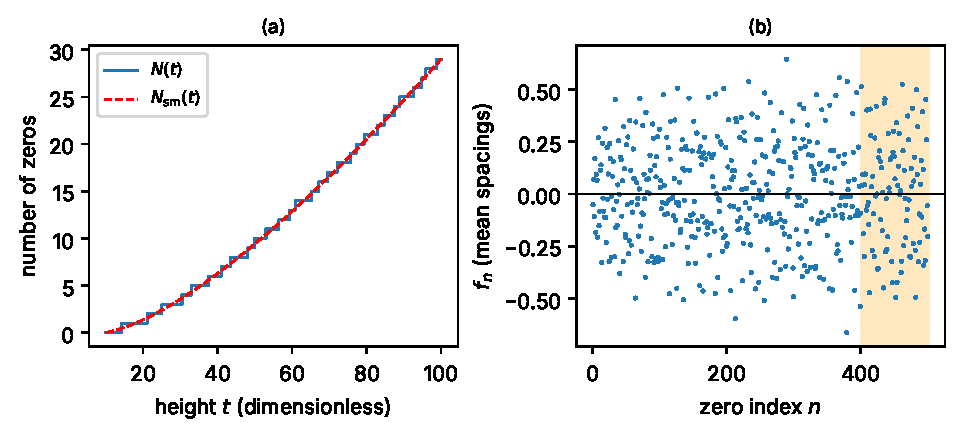
\includegraphics[width=0.95\linewidth]{figs/paper-setup_unfolding.pdf}
\caption{Unfolding. (a) The staircase $N(t)$ of the true zeros and the smooth counting function $\Nsm(t)$ of paper Eq.~(1), for $10\le t\le100$; the staircase crosses the smooth curve repeatedly. (b) The fluctuations $f_n=(t_n-s_n)/\gap_n$ of the first 500 zeros, in units of the local mean spacing. The shaded band marks zeros 401--500, the paper's principal holdout (RE5).}\label{fig:paper-setup-unfolding}
\end{figure}

\subsection{Validating the dataset: the GUE histogram}

The last sentence of Sec.~II~A: ``Unfolded spacings of the first $10^4$ zeros show textbook GUE level repulsion (Fig.~2), confirming the dataset and unfolding.'' Recall from Chapter~\ref{ch:level-statistics} that the unfolded spacing between consecutive zeros is $\Nsm(t_{n+1})-\Nsm(t_n)$, which has mean one by construction, and that the GUE Wigner surmise is
\begin{equation}
p(s)=\frac{32}{\pi^2}\,s^2e^{-4s^2/\pi},
\label{eq:paper-setup-gue}
\end{equation}
against the Poisson law $e^{-s}$ for uncorrelated levels. \Cref{fig:paper-setup-gue} reproduces paper Fig.~2 from the zeros \texttt{qmnt} supplies; the mean unfolded spacing of the first $10^4$ zeros is 1 to better than one part in a thousand. (The sum of the 9999 spacings telescopes to $\Nsm(t_{10000})-\Nsm(t_1)$; writing $\Nsm(t_n)=n-\tfrac12-y_n$ from \eqref{eq:paper-setup-yn}, the mean is exactly $1+(y_1-y_{10000})/9999$, and the computed deviation from 1 is below $10^{-3}$.)

What does this figure prove? Read the paper's verb: ``confirming the dataset and unfolding''. It is a sanity check. Gross errors, such as missed zeros or a wrong density in the unfolding, would typically show up as a non-unit mean or as weight near $s=0$; the check cannot detect every error (a slightly wrong constant in $\Nsm$, or a few slightly perturbed zeros, would leave both features intact). It is not evidence that any particular operator generates the zeros: GUE statistics are shared by vast classes of systems (Chapter~\ref{ch:level-statistics}).

\begin{figure}[htbp]\centering
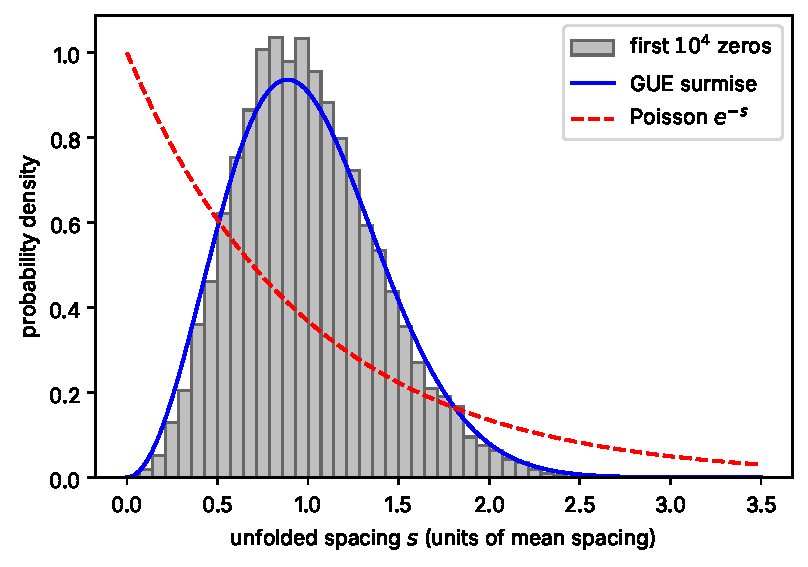
\includegraphics[width=0.85\linewidth]{figs/paper-setup_gue.pdf}
\caption{Reproduction of paper Fig.~2: histogram of the unfolded nearest-neighbour spacings $\Nsm(t_{n+1})-\Nsm(t_n)$ of the first $10^4$ zeros, compared with the GUE Wigner surmise $\frac{32}{\pi^2}s^2e^{-4s^2/\pi}$ and the Poisson law $e^{-s}$. The spacing $s$ is dimensionless (unit mean).}\label{fig:paper-setup-gue}
\end{figure}

\begin{keyideas}
\item Eq.~(1) gives $\Nsm$; smooth zeros solve $\Nsm(s_n)=n-\tfrac12$; the mean spacing is $\gap_n=2\pi/\log(s_n/2\pi)$, eq.~\eqref{eq:paper-setup-gap}.
\item Smooth zeros have the closed Lambert-$W$ form \eqref{eq:paper-setup-lambert} (principal branch).
\item Fluctuations $f_n=(t_n-s_n)/\gap_n$ are what every model predicts; all errors are in mean spacings.
\item The counting residual $y_n$ equals $-f_n$ up to a correction of order $10^{-5}$ to $10^{-3}$, eq.~\eqref{eq:paper-setup-ynfn}.
\item Fig.~2 validates the data and unfolding; it says nothing about which operator, if any, lies behind the zeros.
\end{keyideas}

\section{The background potential and the forward solver}\label{sec:paper-setup-solver}

\subsection{The Wu--Sprung potential, Eq.~(2)}

Sec.~II~B works in units $\hbar=2m=1$, so the Hamiltonian is $H=-d^2/dx^2+V(x)$ and an energy level is directly comparable to a zero height $t$ (Chapter~\ref{ch:schrodinger}). The potential is even, $V(-x)=V(x)$, and is defined implicitly for $V\ge V_0$, $V_0=3.10073\,\pi$, by the paper's Eq.~(2):
\begin{equation}
x(V)=\frac1\pi\Bigl[\sqrt{V-V_0}\,\log\frac{V_0}{2\pi e^2}
+\sqrt V\,\log\frac{\sqrt V+\sqrt{V-V_0}}{\sqrt V-\sqrt{V-V_0}}\Bigr].
\label{eq:paper-setup-ws}
\end{equation}
Chapter~\ref{ch:wu-sprung} derived this from the WKB counting function (Chapter~\ref{ch:wkb}) by an Abel inversion: it is the even, monotone potential whose semiclassical level count equals $\Nsm$. Here we only need to evaluate it.

At $V=V_0$ both terms vanish: $\sqrt{V-V_0}=0$ kills the first, and the second contains $\log(\sqrt{V_0}/\sqrt{V_0})=\log1=0$. So $x(V_0)=0$: the bottom of the well is at the origin. The paper inverts \eqref{eq:paper-setup-ws} ``pointwise by bracketed root finding'' (Appendix~A step~3: Brent's method on a dense reference grid, then cubic-spline interpolation onto the working grid; a cubic spline is a smooth piecewise-cubic curve through the reference points, used to evaluate $V$ between them). Bracketing works because $x(V)$ increases strictly with $V$ (\cref{fig:paper-setup-wusprung}); we prove this after \eqref{eq:paper-setup-wsstable} below.

The second logarithm in \eqref{eq:paper-setup-ws} suffers from cancellation when you evaluate it in floating point (Chapter~\ref{ch:asymptotics}): for large $V$ the denominator $\sqrt V-\sqrt{V-V_0}$ is a small difference of nearly equal numbers. Multiplying top and bottom by $\sqrt V+\sqrt{V-V_0}$ removes it:
\begin{align}
\frac{\sqrt V+\sqrt{V-V_0}}{\sqrt V-\sqrt{V-V_0}}
&=\frac{(\sqrt V+\sqrt{V-V_0})^2}{(\sqrt V-\sqrt{V-V_0})(\sqrt V+\sqrt{V-V_0})}\nonumber\\
&=\frac{(\sqrt V+\sqrt{V-V_0})^2}{V-(V-V_0)}
&&\text{(difference of squares)}\nonumber\\
&=\frac{(\sqrt V+\sqrt{V-V_0})^2}{V_0},\nonumber
\end{align}
so
\begin{equation}
\log\frac{\sqrt V+\sqrt{V-V_0}}{\sqrt V-\sqrt{V-V_0}}=2\log\frac{\sqrt V+\sqrt{V-V_0}}{\sqrt{V_0}} .
\label{eq:paper-setup-wsstable}
\end{equation}

Now the monotonicity. Write $a=\sqrt{V-V_0}$ and $b=\sqrt V$, so that $da/dV=1/(2a)$ and $db/dV=1/(2b)$, and let $c=\log\bigl(V_0/(2\pi e^2)\bigr)$. By \eqref{eq:paper-setup-wsstable}, $\pi x=ac+2b\log\bigl((b+a)/\sqrt{V_0}\bigr)$. Differentiate term by term for $V>V_0$:
\begin{align}
\frac{d(ac)}{dV}&=\frac{c}{2a},\nonumber\\
\frac{d}{dV}\Bigl[2b\log\frac{b+a}{\sqrt{V_0}}\Bigr]&=\frac1b\log\frac{b+a}{\sqrt{V_0}}+2b\,\frac{1/(2b)+1/(2a)}{b+a}
&&\text{(product and chain rules)}\nonumber\\
&=\frac1b\log\frac{b+a}{\sqrt{V_0}}+\frac{(a+b)/a}{a+b}
&&\text{($2b\bigl(\tfrac1{2b}+\tfrac1{2a}\bigr)=1+\tfrac ba$)}\nonumber\\
&=\frac1b\log\frac{b+a}{\sqrt{V_0}}+\frac1a .\nonumber
\end{align}
Adding the two pieces, and using $1+\tfrac c2=1+\tfrac12\log V_0-\tfrac12\log(2\pi)-1=\tfrac12\log\frac{V_0}{2\pi}$,
\begin{equation}
\pi\frac{dx}{dV}=\frac{1}{\sqrt V}\log\frac{\sqrt V+\sqrt{V-V_0}}{\sqrt{V_0}}+\frac{\log(V_0/2\pi)}{2\sqrt{V-V_0}} .
\label{eq:paper-setup-dxdv}
\end{equation}
Both terms are positive for $V>V_0$: the first because $\sqrt V+\sqrt{V-V_0}>\sqrt{V_0}$, the second because $V_0/2\pi=3.10073/2=1.5504>1$. So $x(V)$ is strictly increasing, and its inverse $V(x)$ is well defined for $x\ge0$.

\begin{sample}{Recovering $L=44.883$ from Eq.~(2)}
Scale~1 uses the box $[-L,L]$ with $L=x(V{=}1000)=44.883$ (Sec.~II~B). Verify this number.

\textbf{Step 1: constants.} $V_0=3.10073\pi=9.7412$; $\sqrt{V_0}=3.1211$; $\log\bigl(V_0/(2\pi e^2)\bigr)=\log(9.7412/46.4268)=\log(0.20982)=-1.5615$.

\textbf{Step 2: square roots.} $\sqrt{1000}=31.6228$; $\sqrt{1000-9.7412}=\sqrt{990.2588}=31.4684$.

\textbf{Step 3: first term.} $31.4684\times(-1.5615)=-49.138$.

\textbf{Step 4: second term, stable form.} By \eqref{eq:paper-setup-wsstable}, the logarithm is $2\log\bigl((31.6228+31.4684)/3.1211\bigr)=2\log(20.2145)=2\times3.00640=6.01279$. Times $\sqrt{1000}$: $31.6228\times6.01279=190.141$.

\textbf{Step 5: combine.} $x=(190.141-49.138)/\pi=141.003/\pi=44.883$.
\[
\boxed{L=x(1000)\approx44.883}
\]
The same calculation at $V=1500$ gives the scale-2 half-width $59.957$; Appendix~A step~3 lists the more precise values $44.8827$ and $59.9572$.
\end{sample}

\begin{figure}[htbp]\centering
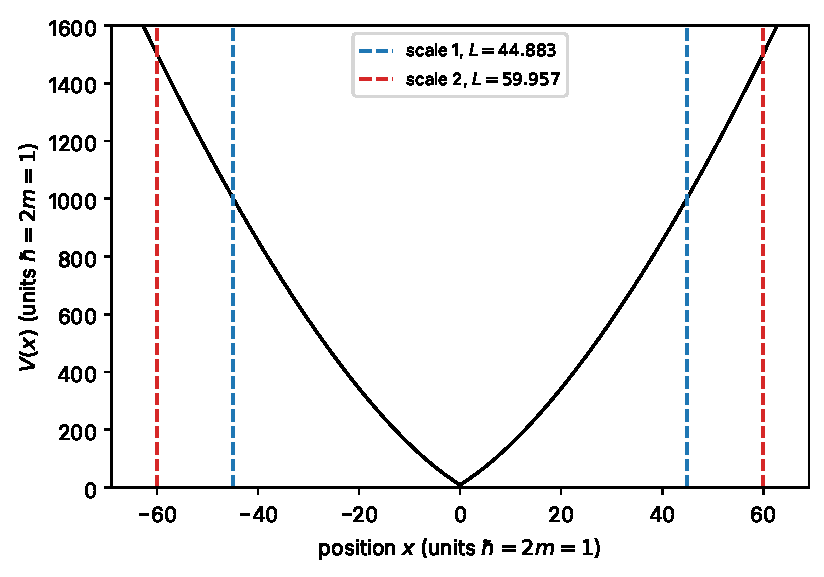
\includegraphics[width=0.85\linewidth]{figs/paper-setup_wusprung.pdf}
\caption{The Wu--Sprung potential of paper Eq.~(2), plotted from its implicit form $x(V)$ and mirrored to $x<0$ because $V$ is even. The bottom is $V_0=3.10073\pi$ at $x=0$. Dashed vertical lines: the box walls at $\pm44.883$ (scale 1, where $V=1000$) and $\pm59.957$ (scale 2, where $V=1500$). Units $\hbar=2m=1$; $x$ and $V$ are dimensionless in these units.}\label{fig:paper-setup-wusprung}
\end{figure}

\subsection{Why 500 and 1000 levels}

Sec.~II~B says scale~1 scores ``the first 500 levels'' and scale~2 ``1000 levels''. The paper does not spell out the reason, so here is our reading, a heuristic based on the turning-point picture of Chapter~\ref{ch:wkb}. A level of energy $E$ is classically confined between turning points $\pm x_E$ with $V(x_E)=E$. If $E<V(L)$ the turning points are inside the box, and the Dirichlet walls at $\pm L$ only touch the exponentially small tail of the wavefunction. At scale~1, $V(L)=1000$, and the 500th zero is $t_{500}=811.18<1000$; at scale~2, $V(L)=1500$, and $t_{1000}=1419.42<1500$. In both cases every scored level has its turning points inside the box. The margin follows from Eq.~(2): at scale~1 the top scored level, $E\approx t_{500}$, turns at $x(811.18)\approx38.53$, about $6.35$ inside the wall at $44.883$; at scale~2 the top level turns at $x(1419.42)\approx57.66$, about $2.29$ inside the wall at $59.957$. The scale-2 margin is smaller, so the argument that the walls touch only a small tail of the wavefunction is strongest at scale~1; we have not quantified the size of that tail. By contrast, $\Nsm(1000)\approx648.6$, so about 649 smooth zeros lie below 1000; levels near the top of that range would feel the walls. Sec.~II~E reports 652 finite-difference states with $E\le1000$, close to this smooth count.

\subsection{The finite-difference solver}

Appendix~A steps 3--4 and Sec.~II~B: the interval $(-L,L)$ carries $N$ uniform interior points with spacing $h=2L/(N+1)$ and Dirichlet walls (Chapter~\ref{ch:finite-differences}). The second-order difference gives a symmetric tridiagonal matrix with diagonal $2/h^2+V_j$ and off-diagonal $-1/h^2$; its eigenpairs come from LAPACK through \texttt{eigh\_tridiagonal} (Chapter~\ref{ch:eigen}), restricted to an energy range: $[0,900]$ for the Hermitian work at scale~1, $[0,1000]$ for the non-Hermitian tensors (652 states), $[0,1500]$ at scale~2 (1079 states). The working grid has $N=6000$ at scale~1 and $N=8000$ at scale~2; both give $h\approx0.0150$.

\subsection{Removing the discretization bias}

Chapter~\ref{ch:finite-differences} showed that the finite-difference eigenvalues of $-d^2/dx^2$ lie below the continuum ones by an amount that grows with energy (dispersion). For the levels the paper scores this matters a great deal.

\begin{sample}{How large is the dispersion error?}
Consider the empty box ($V=0$, RE3) on $[-44.883,44.883]$ with the scale-1 working grid $N=6000$. Find the level $k$ with continuum energy near 700 and compare its discrete eigenvalue with the continuum value. Express the shortfall in mean spacings of the zeros at height 700.

\textbf{Step 1: grid spacing.} $h=2L/(N+1)=89.766/6001=0.0149585$.

\textbf{Step 2: choose $k$.} Continuum levels are $E_k=(k\pi/2L)^2$ (Chapter~\ref{ch:bound-states}). Setting $E_k=700$ gives $k=2L\sqrt{700}/\pi=755.98$; take $k=756$, for which $E_{756}=(756\pi/89.766)^2=(26.4582)^2=700.03$.

\textbf{Step 3: discrete eigenvalue.} From Chapter~\ref{ch:finite-differences}, $E_k^{\rm disc}=\frac{4}{h^2}\sin^2\frac{k\pi h}{4L}$. Since $h/(4L)=1/(2(N+1))$, the angle is $\theta=k\pi/(2(N+1))=2375.04/12002=0.197887$. Then $\sin\theta=0.196598$, $\sin^2\theta=0.0386509$, $4/h^2=17876.5$, and $E^{\rm disc}_{756}=690.94$.

\textbf{Step 4: shortfall.} $700.03-690.94=9.09$. The mean spacing of the zeros at $t=700$ is $2\pi/\log(700/2\pi)=1.333$, so the shortfall is $9.09/1.333=6.8$ spacings.
\[
\boxed{E^{\rm disc}_{756}\approx690.94\ \text{vs}\ E_{756}\approx700.03:\ \text{short by}\approx9.09\approx6.8\ \text{spacings}}
\]
In the Wu--Sprung potential we expect the bias at a given energy to be smaller. Heuristically (we do not derive this here), the leading error is proportional to $h^2$ times the average of $k(x)^4=(E-V(x))^2$ over the state, where $k(x)$ is the local WKB wavenumber of Chapter~\ref{ch:wkb}, and in a well this average is smaller than $E^2$. The paper reports that at levels 401--500 on the working grid the dispersion ``reaches two mean spacings'' (Sec.~II~C, ``No leakage''). Either way, it is far larger than the 0.263-spacing fluctuations the models are trying to predict.
\end{sample}

The paper's remedy is to correct the \emph{targets}, not the operator. Compute the smooth potential's eigenvalues $E_n^{\rm g}[\text{smooth}]$ on the working grid, and also a Richardson extrapolation $E_n^{\rm Rich}[\text{smooth}]$ from a finer pair of grids (Appendix~A step~3: $N=12000/24000$ at scale~1, $16000/32000$ at scale~2). The grid bias of level $n$ is
\begin{equation}
\Delta_n=E_n^{\rm g}[\text{smooth}]-E_n^{\rm Rich}[\text{smooth}],
\label{eq:paper-setup-delta}
\end{equation}
and the bias-corrected targets are (Sec.~II~B; Appendix~A step~5)
\begin{equation}
\tilde t_n=t_n+\Delta_n .
\label{eq:paper-setup-target}
\end{equation}
The idea: the working-grid eigenvalue of \emph{any} nearby potential is low by roughly $\Delta_n$, so the fit should aim at $t_n$ shifted down by the same amount ($\Delta_n<0$), not at $t_n$ itself.

The paper reports the quality of the extrapolant: the residual of $E^{\rm Rich}$ against the smooth zeros is $0.005$ spacings on average and $0.063$ at most, ``worst at low $n$, the known semiclassical weakness of the construction'' (Sec.~II~B; Appendix~A gives the same values at scale~2). Recall from Chapter~\ref{ch:wkb} that WKB counting is least accurate for the lowest levels; since Eq.~(2) is built to make the \emph{WKB} count equal $\Nsm$, the true low levels deviate slightly from $s_n$.

\begin{sample}{Reading the Richardson formula correctly}
Sec.~II~B writes $E^{\rm Rich}=(4E_{2h}-E_h)/3$. Test the two possible readings of the subscript on a model with exactly quadratic error, $E_h=E+ah^2$, with $E=100$, $a=-50$, $h=0.02$.

\textbf{Step 1: the standard form.} Chapter~\ref{ch:finite-differences} derived $(4E_{h/2}-E_h)/3$, where $h/2$ is the \emph{finer} grid. Here $E_h=100-50(0.0004)=99.98$ and $E_{h/2}=100-50(0.0001)=99.995$, so $(4\times99.995-99.98)/3=(399.98-99.98)/3=100.000$, exact.

\textbf{Step 2: literal reading with spacing $2h$.} $E_{2h}=100-50(0.0016)=99.92$, and $(4\times99.92-99.98)/3=(399.68-99.98)/3=99.900$. In general, $(4E_{2h}-E_h)/3=E+5ah^2$: the error is amplified fivefold.
\[
\boxed{\text{finer-grid reading: }100.000\ (\text{exact});\qquad \text{spacing-}2h\text{ reading: }99.900}
\]
So the weight 4 must multiply the eigenvalue on the finer grid: only then does the $h^2$ error cancel. The paper's subscript ``$2h$'' must therefore be read as ``the grid with twice the points''. Appendix~A step~3 lists the Richardson pairs $12000/24000$ and $16000/32000$, consistent with that reading. With $h=2L/(N+1)$, doubling $N$ halves $h$ only approximately: $h_{24000}/h_{12000}=12001/24001=\tfrac12(1+\eta)$ with $\eta=1/24001\approx4.2\times10^{-5}$ (smaller still for the scale-2 pair). Repeating Step~2 with $h/2$ replaced by $h(1+\eta)/2$ gives $E+\tfrac{2\eta+\eta^2}{3}\,ah^2\approx E+2.8\times10^{-5}\,ah^2$, a negligible residual compared with the coarse-grid error $ah^2$. The extrapolation is from the finer pair, and the working grid ($6000$ or $8000$) is a third, coarser grid.
\end{sample}

\begin{pitfall}
Three different grids appear at each scale: the working grid on which all fitting runs, and a finer pair used only for Richardson extrapolation. $\Delta_n$ compares the working grid with the extrapolant from the finer pair. Do not confuse it with the difference between the two finer grids.
\end{pitfall}

\begin{keyideas}
\item Eq.~(2) defines the even Wu--Sprung potential implicitly; $x(V_0)=0$, $L=x(1000)=44.883$, $x(1500)=59.957$; use the stable form \eqref{eq:paper-setup-wsstable} numerically.
\item Every scored level has its turning points inside the box (our reading of why 500 and 1000 levels are scored).
\item Finite-difference dispersion at the scored levels is several times larger than the fluctuations; the paper removes it from the targets, $\tilde t_n=t_n+\Delta_n$.
\item Richardson extrapolation uses the finer grid of a doubling pair; read the paper's subscript accordingly.
\end{keyideas}

\section{The Hermitian fit and the out-of-sample protocol}\label{sec:paper-setup-protocol}
% DYK-BEGIN
\begin{didyouknow}{Leave Some Data Out}
Cross-validation judges a model on data it never saw while fitting. It was formalized in the mid-1970s by the statisticians Mervyn Stone and Seymour Geisser, building on older practice of holding out samples. The idea is simple and powerful. A fit can always be made to match its own training data, so only performance on fresh data measures real predictive skill.
\end{didyouknow}
% DYK-END

\subsection{The model and the fit}

Sec.~II~C perturbs the background, $V\to V+\delta V$, with
\begin{equation}
\delta V(x)=\sum_{k=0}^{M-1}c_k\cos\frac{k\pi x}{L},
\label{eq:paper-setup-dv}
\end{equation}
an even function (Chapter~\ref{ch:fourier-series}) with $M$ coefficients $c_k$. The fit is iterated linearization, which Chapter~\ref{ch:fitting} developed in full. In outline (Appendix~A step~6):
\begin{enumerate}
\item Solve for eigenpairs $(E_n,\psi_n)$ of the current potential on the working grid.
\item Form residuals $r_n=\tilde t_n-E_n$ on the training indices and the sensitivity matrix $A_{nk}=\int|\psi_n|^2\cos(k\pi x/L)\,dx$ (the first-order energy shift per unit $c_k$; Chapter~\ref{ch:perturbation}).
\item Propose $c\mathrel{+}=V\,\mathrm{diag}\bigl(\sigma/(\sigma^2+\lambda\sigma_1^2)\bigr)U^\top r$, an SVD-damped least-squares step (Chapter~\ref{ch:least-squares}). Here $U,\sigma,V$ come from the SVD of $A$ (this $V$ is the matrix of right singular vectors, not the potential), $\sigma_1$ is the largest singular value and $\lambda$ the Levenberg--Marquardt damping.
\item Try $\lambda$ from the list $(0.2\lambda,\lambda,5\lambda,25\lambda)$; accept a step only if the new rms is below $0.999$ times the old one (the scale-2, $M=300$ row of Table~I used $1-10^{-5}$ instead, as its caption notes); on success set $\lambda\leftarrow\max(0.5\lambda_{\rm acc},10^{-7})$, on total failure $\lambda\leftarrow30\lambda$; stop at $\lambda>10^4$. The ridge variant adds $\mu\sigma_1^2$ to the denominator.
\end{enumerate}
The protocol is deterministic from $c=0$; optimizer variability is probed with random initial $c$.

\paragraph{Other bases.} The same protocol runs with two alternative even bases: Chebyshev polynomials $T_k(2|x|/L-1)$, $k=0,\dots,M-1$, where $T_k(u)=\cos(k\arccos u)$ for $-1\le u\le1$ (so $u=-1$ at $x=0$ and $u=1$ at $|x|=L$, with resolution concentrated near both ends), and piecewise-linear ``hat'' functions on $M$ uniform nodes of $|x|/L$, each nonzero only between its two neighbouring nodes. ``Only the basis changes.'' Chapter~\ref{ch:fitting} plotted all three.

\subsection{Out-of-sample scoring}

The crucial step is Appendix~A step~7: fit on zeros $1,\dots,n_{\rm fit}$ only, then perform ``a single plain eigensolve of the fitted potential'', and score it on the held-out zeros. No further adjustment happens after the fit.

Two numbers are reported. Let $\mathcal T$ be the set of held-out indices, with $n_{\rm test}$ members. Let $\hat t_n$ be a model's predicted height for zero $n$, $t_n$ the true height, and $R_n$ a reference (the model's smooth baseline). Define the predicted and true fluctuations relative to the reference,
\begin{equation}
\hat f_n=\frac{\hat t_n-R_n}{\gap_n},\qquad f^{\rm ref}_n=\frac{t_n-R_n}{\gap_n}.
\label{eq:paper-setup-pq}
\end{equation}
Then
\begin{equation}
\rms=\Bigl[\frac{1}{n_{\rm test}}\sum_{n\in\mathcal T}\Bigl(\frac{\hat t_n-t_n}{\gap_n}\Bigr)^2\Bigr]^{1/2}=\Bigl[\frac{1}{n_{\rm test}}\sum_{n\in\mathcal T}(\hat f_n-f^{\rm ref}_n)^2\Bigr]^{1/2},
\qquad
\corr=\text{Pearson}(\hat f,f^{\rm ref}),
\label{eq:paper-setup-score}
\end{equation}
where the second form of the rms follows because $\hat f_n-f^{\rm ref}_n=(\hat t_n-t_n)/\gap_n$, the reference cancelling. (We write $\mathcal T$, $n_{\rm test}$ and hats to avoid clashes with the Hamiltonian $H$, the number $K$ of frequencies in control C2, the prime set $P$ and the prime $p$.) For the oracle, $\hat t_n$ solves the level equation of \cref{sec:paper-setup-oracle} and $R_n=s_n$. For the operator, the fit is scored against $\tilde t_n$, which plays the role of the true height, with the reference $E_n^{\rm g}[\text{smooth}]$ (``both measured relative to the unperturbed smooth-potential levels'', Sec.~II~C). Writing $E^{\rm g}_n$ and $E^{\rm Rich}_n$ for the smooth-potential eigenvalues on the working grid and from Richardson extrapolation, and $\Delta_n=E^{\rm g}_n-E^{\rm Rich}_n$ for the grid bias \eqref{eq:paper-setup-delta}, this is the same as using the corrected prediction $\hat t_n=E_n[\text{fit}]-\Delta_n$ and the reference $R_n=E^{\rm Rich}_n$ against the raw zeros, because both fluctuations are unchanged:
\begin{align}
\bigl(E_n[\text{fit}]-\Delta_n\bigr)-E^{\rm Rich}_n
&=E_n[\text{fit}]-E^{\rm g}_n+E^{\rm Rich}_n-E^{\rm Rich}_n=E_n[\text{fit}]-E^{\rm g}_n,
&&\text{(insert $\Delta_n$)}\nonumber\\
t_n-E^{\rm Rich}_n
&=t_n+\Delta_n-E^{\rm g}_n=\tilde t_n-E^{\rm g}_n
&&\text{(add and subtract $E^{\rm g}_n$; $\tilde t_n=t_n+\Delta_n$)}.\nonumber
\end{align}
Dividing by $\gap_n$ shows that the predicted and true fluctuations, and hence both scores, are the same in the two descriptions. Recall from Chapter~\ref{ch:probability} why both numbers are needed: rms measures size of error, correlation measures shape agreement. A prediction with the right shape but the wrong amplitude can have high correlation and a poor rms.

\subsection{The splits}

The paper uses four kinds of train/test split (\cref{fig:paper-setup-splits}).
\begin{enumerate}
\item \textbf{Forward} (the main protocol): train on zeros $1,\dots,n_{\rm fit}$, test on the next window, e.g.\ $1$--$400\to401$--$500$ at scale~1 and $1$--$800\to801$--$1000$ at scale~2 (Table~I).
\item \textbf{Within-height random} (Sec.~II~C, ``Within-height splits''): inside zeros 1--400 (scale~1) or 1--800 (scale~2), hold out a random 20\%; ten seeds at scale~1, two at scale~2 (Appendix~A step~17: \texttt{rng.choice(n, n/5, replace=False)}, residuals restricted to training indices).
\item \textbf{Odd/even}: train on odd-indexed zeros and score the even ones, and vice versa.
\item \textbf{Interpolation} (Sec.~III; Appendix~A step~14): train on $1$--$200\cup301$--$500$, predict the gap $201$--$300$.
\end{enumerate}
Why within-height splits at all? Because forward splits put the test zeros higher up, where the fluctuation amplitude is slightly larger; the paper notes that the null grows from 0.263 to 0.296 over Table~V. A model could fail forward because the test data come from a different region (covariate shift, Chapter~\ref{ch:generalization}) rather than because it learned nothing. Within-height splits remove that excuse.

\begin{figure}[htbp]\centering
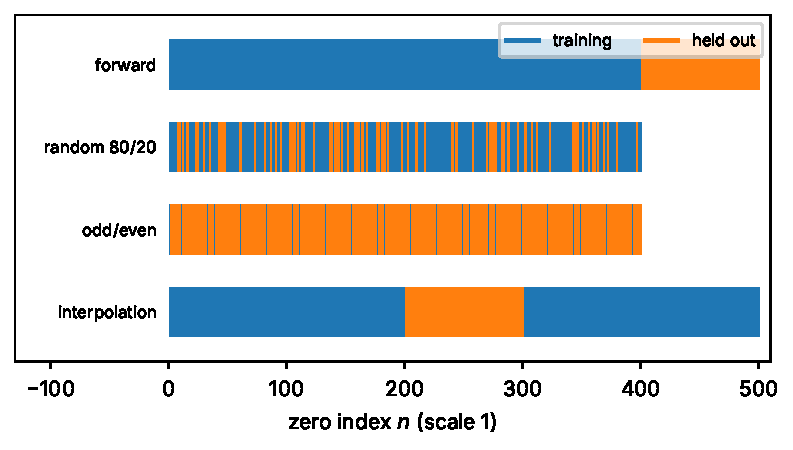
\includegraphics[width=0.95\linewidth]{figs/paper-setup_splits.pdf}
\caption{The four train/test designs of the paper, drawn along the zero index $n$ at scale 1. Blue: training zeros; orange: held-out zeros. Forward split (Table~I), within-height random 80/20 split (one seed shown; Table~III), odd/even split (Table~III), and the interpolation split of Sec.~III.}\label{fig:paper-setup-splits}
\end{figure}

\begin{checkpoint}
In an odd/even split at scale 1, the model trains on 200 levels. The caption of Table~III describes the odd/even rows with $M$ at or above the number of training levels (here $M\ge200$) as ``saturated''. Using Chapter~\ref{ch:least-squares}, say briefly why.
\end{checkpoint}
\checkanswer{With $M$ at or above the number of training levels (200 here), the model has at least as many adjustable numbers as data, so counting alone no longer prevents an exact fit (Chapter~\ref{ch:least-squares}: a square or underdetermined linear system can generically be solved exactly). In practice exactness also requires the basis to cover the levels and the nonlinear iteration to converge (Chapter~\ref{ch:fitting}): Table~III shows in-sample rms 0.176 and 0.171 at $M=200$ but $<10^{-3}$ at $M=400$. Either way, a small in-sample error in these rows says nothing about predictive skill.}

\begin{keyideas}
\item The fitted correction $\delta V=\sum c_k\cos(k\pi x/L)$ is fit by SVD-damped Levenberg--Marquardt steps that are accepted only if they improve the rms.
\item Out-of-sample scoring is a single plain eigensolve of the fitted potential, scored on zeros never used in fitting.
\item rms and correlation of predicted versus true fluctuations, eq.~\eqref{eq:paper-setup-score}; the rms does not depend on the reference, the correlation does (Problem~19).
\item Forward, within-height random, odd/even and interpolation splits separate ``learned nothing'' from ``tested elsewhere''.
\end{keyideas}

\section{Two nulls and the leakage argument}\label{sec:paper-setup-nulls}

\subsection{Why a null model}

An rms of $0.3$ spacings is meaningless on its own. Is that good? It depends on how large the thing you are predicting is. The \emph{null} model predicts no fluctuation at all, $\hat t_n=R_n$, so $\hat f_n=0$ and, by \eqref{eq:paper-setup-score},
\begin{equation}
\rms_{\rm null}=\Bigl[\frac{1}{n_{\rm test}}\sum_{n\in\mathcal T}\bigl(f^{\rm ref}_n\bigr)^2\Bigr]^{1/2},
\label{eq:paper-setup-null}
\end{equation}
the rms size of the true fluctuations themselves. A model has predictive skill only if its rms is below this and its correlation is positive. Every claim in Tables~I--V is relative to the null.

\begin{pitfall}
The null has no correlation: its predicted fluctuations $\hat f_n$ are all zero, a sequence with zero variance, so the Pearson coefficient (covariance divided by the product of standard deviations, Chapter~\ref{ch:probability}) has zero in the denominator. Do not look for a ``null corr'' column in the tables; there is none.
\end{pitfall}

\subsection{The two nulls}

The paper has two families of models, and each has its own smooth baseline.
\begin{itemize}
\item \textbf{Operator null:} the unperturbed Wu--Sprung potential, $\delta V=0$. Its prediction for zero $n$ is its own eigenvalue.
\item \textbf{Oracle null:} the smooth zeros $s_n$, the solutions of the mean counting equation \eqref{eq:paper-setup-sn}.
\end{itemize}
These are ``conceptually distinct (an eigenvalue spectrum versus the solution of the mean counting function)'' (Sec.~II~C). Yet ``numerically its holdout error coincides with that of the smooth zeros used as the oracle's null (both $0.2631$ on zeros 401--500), so the operator and oracle comparisons share one effective baseline.'' Let us see exactly why.

Score the unperturbed potential by the operator protocol: prediction $E_n^{\rm g}[\text{smooth}]$ against target $\tilde t_n$. The error in height units is
\begin{align}
\tilde t_n-E_n^{\rm g}[\text{smooth}]
&=t_n+\Delta_n-E_n^{\rm g}[\text{smooth}]
&&\text{(by \eqref{eq:paper-setup-target})}\nonumber\\
&=t_n+E_n^{\rm g}[\text{smooth}]-E_n^{\rm Rich}[\text{smooth}]-E_n^{\rm g}[\text{smooth}]
&&\text{(by \eqref{eq:paper-setup-delta})}\nonumber\\
&=t_n-E_n^{\rm Rich}[\text{smooth}]. \label{eq:paper-setup-opnull}
\end{align}
The working-grid eigenvalue cancels completely. The operator null is the error of the Richardson-extrapolated (essentially continuum) spectrum of the smooth potential against the raw zeros. Now write $\varepsilon_n=(E^{\rm Rich}_n[\text{smooth}]-s_n)/\gap_n$ for the residual the paper reports (mean 0.005, max 0.063 spacings). Dividing \eqref{eq:paper-setup-opnull} by $\gap_n$,
\begin{equation}
\frac{t_n-E_n^{\rm Rich}}{\gap_n}=\frac{t_n-s_n}{\gap_n}-\frac{E_n^{\rm Rich}-s_n}{\gap_n}=f_n-\varepsilon_n .
\label{eq:paper-setup-twonulls}
\end{equation}
The oracle null error is $f_n$; the operator null error is $f_n-\varepsilon_n$.

How different can their rms values be? Write $\rms(a)=\norm{a}/\sqrt{n_{\rm test}}$ with $\norm{\cdot}$ the Euclidean norm of an $n_{\rm test}$-component vector (Chapter~\ref{ch:linear-algebra}). We need the triangle inequality $\norm{a+b}\le\norm a+\norm b$. It follows from the Cauchy--Schwarz inequality $a\cdot b\le\norm a\,\norm b$ (Chapter~\ref{ch:probability}):
\begin{align}
\norm{a+b}^2&=\norm a^2+2\,a\cdot b+\norm b^2 &&\text{(expand the dot product)}\nonumber\\
&\le\norm a^2+2\norm a\,\norm b+\norm b^2 &&\text{(Cauchy--Schwarz)}\nonumber\\
&=(\norm a+\norm b)^2,\nonumber
\end{align}
and taking square roots of the two nonnegative sides gives the inequality. Applied twice, it gives
\begin{align}
\norm f&=\norm{(f-\varepsilon)+\varepsilon}\le\norm{f-\varepsilon}+\norm{\varepsilon},\nonumber\\
\norm{f-\varepsilon}&=\norm{f+(-\varepsilon)}\le\norm f+\norm{\varepsilon}.\nonumber
\end{align}
The first line says $\norm f-\norm{f-\varepsilon}\le\norm\varepsilon$, the second says $\norm{f-\varepsilon}-\norm f\le\norm\varepsilon$; together,
\begin{equation}
\bigl|\rms(f-\varepsilon)-\rms(f)\bigr|\le\rms(\varepsilon)\le\max_n|\varepsilon_n| .
\label{eq:paper-setup-rmsbound}
\end{equation}
The last inequality holds because a mean of squares cannot exceed the largest square. With the paper's $\max|\varepsilon_n|=0.063$, the two nulls can differ by at most $0.063$ on any holdout. On zeros 401--500 they agree to four digits. This is consistent with $\varepsilon_n$ being much smaller there than its worst value (the paper says the worst residuals occur at low $n$), although agreement of the rms values alone does not prove it: expanding the squares, $\rms(f-\varepsilon)^2-\rms(f)^2=\overline{\varepsilon^2}-2\,\overline{f\varepsilon}$ (bars denote averages over the holdout), so an $\varepsilon$ that is uncorrelated with $f$ changes the rms only through the second-order term $\overline{\varepsilon^2}$.

\begin{sample}{The rms bound on a small example}
Let $f=(0.30,-0.20,0.10,-0.40)$ and $\varepsilon=(0.010,-0.020,0.005,0.015)$ (illustrative numbers, not the paper's). Check \eqref{eq:paper-setup-rmsbound}.

\textbf{Step 1: $\rms(f)$.} $(0.09+0.04+0.01+0.16)/4=0.075$, so $\rms(f)=0.2739$.

\textbf{Step 2: $\rms(f-\varepsilon)$.} $f-\varepsilon=(0.290,-0.180,0.095,-0.415)$; squares sum to $0.0841+0.0324+0.009025+0.172225=0.29775$; divided by 4 gives $0.074438$, so $\rms=0.2728$.

\textbf{Step 3: $\rms(\varepsilon)$.} Squares sum to $0.00075$; divided by 4 gives $0.0001875$; $\rms(\varepsilon)=0.0137$.

\textbf{Step 4: compare.} $|0.2728-0.2739|=0.0010\le0.0137\le0.020=\max|\varepsilon_n|$.
\[
\boxed{|\Delta\rms|\approx0.0010\ \le\ \rms(\varepsilon)\approx0.0137\ \le\ \max|\varepsilon_n|=0.020}
\]
The difference of the rms values is much smaller than the bound, because $\varepsilon$ is not aligned with $f$.
\end{sample}

\subsection{No leakage through the bias correction}

Here is a subtle point a referee would raise. The corrected targets $\tilde t_n=t_n+\Delta_n$ are formed for \emph{all} $n$, including held-out ones. Does the held-out information leak into the fit through them? The paper's answer is its Eq.~(3):
\begin{equation}
\tilde t_n-E_n[\text{fit}]=t_n-\bigl(E_n[\text{fit}]-\Delta_n\bigr).
\label{eq:paper-setup-leak}
\end{equation}
Derivation, one line at a time:
\begin{align}
\tilde t_n-E_n[\text{fit}]&=(t_n+\Delta_n)-E_n[\text{fit}] &&\text{(definition \eqref{eq:paper-setup-target})}\nonumber\\
&=t_n-E_n[\text{fit}]+\Delta_n &&\text{(rearrange)}\nonumber\\
&=t_n-\bigl(E_n[\text{fit}]-\Delta_n\bigr) &&\text{(factor the minus sign)}.\nonumber
\end{align}
So scoring the fit against $\tilde t_n$ is algebraically identical to correcting the \emph{prediction} by $\Delta_n$ and scoring against the raw zeros.

The identity by itself proves nothing about leakage; it is true for any $\Delta_n$ whatsoever. What carries the argument is the second half of the paragraph: $\Delta_n$ ``is built solely from eigenvalues of the \emph{unperturbed} potential on two grids; no zero, in-sample or held-out, enters it.'' Look at \eqref{eq:paper-setup-delta}: both terms are eigenvalues of the smooth potential, which is fixed by $\Nsm$ alone. So $\Delta_n$ is a known, data-free correction to the solver, exactly like a calibration constant of an instrument. The identity shows that applying it to the targets is the same as applying it to the predictions; the construction shows it contains no information about any zero. Both halves are needed (Problem~7 asks you to see what would go wrong if the second half failed).

Why bother with the correction at all? Because without it, finite-difference dispersion ``at levels 401--500 on the working grid reaches two mean spacings and would otherwise dominate both the null and every model identically''. Appendix~A's anchors quantify this: the raw-zero null on the uncorrected working grid is $2.09$ on zeros 401--500, against $0.2631$ after correction. A null of 2.09 would make every model look equally terrible and hide all differences between them.

\begin{sample}{The leakage identity with numbers}
Take illustrative values (not from the paper) for one held-out level: $t_n=700.250$, $E^{\rm g}_n[\text{smooth}]=698.300$, $E^{\rm Rich}_n[\text{smooth}]=700.100$, and a fitted prediction $E_n[\text{fit}]=698.600$. Compute the error both ways, and the null error.

\textbf{Step 1: bias.} $\Delta_n=698.300-700.100=-1.800$.

\textbf{Step 2: corrected target.} $\tilde t_n=700.250-1.800=698.450$.

\textbf{Step 3: score against the corrected target.} $\tilde t_n-E_n[\text{fit}]=698.450-698.600=-0.150$.

\textbf{Step 4: score the corrected prediction against the raw zero.} $E_n[\text{fit}]-\Delta_n=698.600+1.800=700.400$; $t_n-700.400=-0.150$. Same, as \eqref{eq:paper-setup-leak} demands.

\textbf{Step 5: null error.} By \eqref{eq:paper-setup-opnull}, $t_n-E^{\rm Rich}_n=700.250-700.100=0.150$.
\[
\boxed{\tilde t_n-E_n[\text{fit}]=t_n-(E_n[\text{fit}]-\Delta_n)=-0.150;\qquad \text{null error}=+0.150}
\]
In this illustration the fit predicts a fluctuation of $E_n[\text{fit}]-E^{\rm g}_n[\text{smooth}]=+0.300$ where the true one is $\tilde t_n-E^{\rm g}_n[\text{smooth}]=+0.150$: right sign, twice the size, so its error ($0.150$ in magnitude) is no smaller than the null's.
\end{sample}

A second leakage safeguard appears in Appendix~A step~20 for the sinusoidal controls: ``Overwriting held-out data with noise before fitting leaves all fitted coefficients bit-identical.'' This is the strongest kind of leakage test: physically destroy the held-out data and confirm that nothing in the fit changes.

\begin{checkpoint}
Does the operator null on zeros 401--500 depend on the working grid size $N=6000$? Use \eqref{eq:paper-setup-opnull}.
\end{checkpoint}
\checkanswer{No. The working-grid eigenvalue cancels, leaving $t_n-E^{\rm Rich}_n$, which depends only on the finer Richardson pair. Changing the working grid changes $\Delta_n$ and the fitted eigenvalues together.}

\begin{keyideas}
\item Every skill claim is relative to a null; the null rms is the rms of the true fluctuations, and the null has no correlation.
\item The operator null equals $t_n-E^{\rm Rich}_n[\text{smooth}]$, eq.~\eqref{eq:paper-setup-opnull}; it differs from the smooth-zero null by at most $\max|\varepsilon_n|=0.063$, eq.~\eqref{eq:paper-setup-rmsbound}, and coincides with it numerically (0.2631, a coincidence of measured values, not an identity) on zeros 401--500.
\item No leakage: Eq.~(3) shows correcting targets equals correcting predictions, and $\Delta_n$ contains no zero.
\item Without the correction the null on 401--500 would be 2.09 instead of 0.263.
\end{keyideas}

\section{The arithmetic oracle and the fitted sinusoidal controls}\label{sec:paper-setup-oracle}

\subsection{The oracle, Eq.~(4)}

Sec.~II~D's prediction baseline is the paper's Eq.~(4),
\begin{equation}
\Nfl(t)=-\frac1\pi\sum_{p\in P}\sum_{m=1}^{3}\frac{\sin(mt\log p)}{m\,p^{m/2}},
\label{eq:paper-setup-oracle}
\end{equation}
for a finite prime set $P$, with predicted zeros solving
\begin{equation}
\Nsm(t)+\Nfl(t)=n-\tfrac12 .
\label{eq:paper-setup-level}
\end{equation}
Chapter~\ref{ch:explicit-formula} derived \eqref{eq:paper-setup-oracle} from the Euler product: $\log\zeta(s)=\sum_p\sum_m p^{-ms}/m$ for $\Re s>1$, and the imaginary part formally continued to $s=\tfrac12+it$ gives $S(t)\approx-\frac1\pi\sum_p\sum_m\sin(mt\log p)/(mp^{m/2})$, using $p^{-ms}=p^{-m\sigma}e^{-imt\log p}$ (Chapter~\ref{ch:complex}). Each prime contributes oscillations of angular frequency $m\log p$ in $t$; for $p=2$ the period is $2\pi/\log2\approx9.065$ (RE2).

\begin{beyond}
The full series over all primes does not converge on the critical line, so \eqref{eq:paper-setup-oracle} is a heuristic truncation, not a convergent approximation with a proved error bound. Rigorous explicit formulae (Riemann--von Mangoldt, Guinand--Weil) relate smoothed sums over zeros to smoothed sums over prime powers; see \cite{edwards,titchmarsh,davenport}. That truncations such as \eqref{eq:paper-setup-oracle} predict individual zeros well at these heights is a numerical observation, which Table~V documents and which Fran\c{c}a and LeClair \cite{francaleclair,leclair} studied.
\end{beyond}

Three features of the oracle matter for reading the paper.
\begin{enumerate}
\item \textbf{Zero fitted parameters.} Nothing in \eqref{eq:paper-setup-oracle} or \eqref{eq:paper-setup-level} is adjusted to any zero. Every zero is held out.
\item \textbf{Not a fair competitor.} The paper says so: ``It is not a fair ML competitor (it encodes the known functional form); its role is informational, to prove that transferable structure about unseen zeros exists and to quantify how much of it simple arithmetic captures.''
\item \textbf{Root finding.} Appendix~A step~8 solves \eqref{eq:paper-setup-level} by Brent's method (Chapter~\ref{ch:asymptotics}) ``bracketed $\pm3$ around the smooth zero (bracket expanded on sign failure)''. The step does not state the unit of the $\pm3$; \texttt{qmnt.oracle\_zeros} uses three local mean spacings.
\end{enumerate}

\begin{sample}{Reproducing two entries of Table~V}
Compute the oracle's rms and correlation on zeros 401--500 with $P=\{2\}$ and with the first six primes, and compare with Table~V.

\textbf{Step 1: data.} Indices $n=401,\dots,500$; true heights from \texttt{qmnt.zeros(500)}.

\textbf{Step 2: predictions.} \texttt{qmnt.oracle\_zeros(n, primes)} solves \eqref{eq:paper-setup-level} for each $n$ with $m\le3$.

\textbf{Step 3: score.} \texttt{qmnt.score(t\_pred, n)} returns the rms of $(\hat t_n-t_n)/\gap_n$ and the Pearson correlation of $\hat f_n=(\hat t_n-s_n)/\gap_n$ with $f^{\rm ref}_n=f_n$, as in \eqref{eq:paper-setup-score} with $R_n=s_n$.

\textbf{Step 4: results.} One prime gives rms $0.198$, corr $+0.66$; six primes give $0.074$, $+0.96$. Both match Table~V's 401--500 row.
\[
\boxed{\{2\}:\ 0.198/{+0.66};\qquad \{2,3,5,7,11,13\}:\ 0.074/{+0.96}\qquad(\text{null }0.263)}
\]
A single prime, with nothing fitted, already beats the null by a quarter.
\end{sample}

\begin{pycode}
import numpy as np, qmnt

n = np.arange(401, 501)                  # RE5: principal holdout
t_true = qmnt.zeros(500)[n - 1]
null = qmnt.rms(qmnt.fluct(t_true, n))   # about 0.263

for k in [1, 3, 6, 25]:
    P = qmnt.first_primes(k)
    t_pred = qmnt.oracle_zeros(n, P, mmax=3)
    r, c = qmnt.score(t_pred, n)
    print(k, "primes: rms", round(r, 3), "corr", round(c, 2),
          "null", round(null, 3))
\end{pycode}

\Cref{fig:paper-setup-oracle} shows the oracle half of paper Fig.~1. The true fluctuation and the six-prime prediction are plotted for zeros 370--460; nothing changes at the boundary $n=400$ because the oracle never saw any zero.

\begin{figure}[htbp]\centering
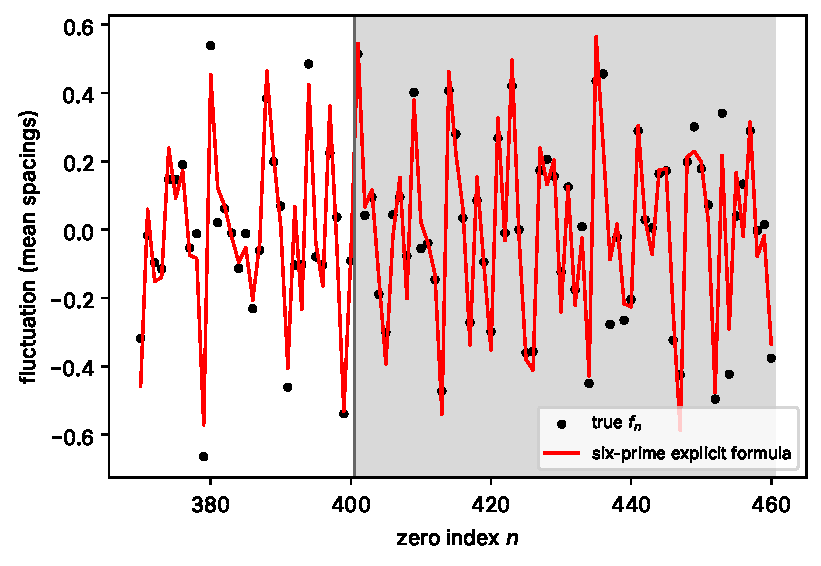
\includegraphics[width=0.85\linewidth]{figs/paper-setup_oracle.pdf}
\caption{The oracle half of paper Fig.~1: true fluctuations $f_n=(t_n-s_n)/\gap_n$ of zeros 370--460 (dots) and the six-prime explicit-formula prediction of paper Eq.~(4) (line), both in units of the local mean spacing. The shaded region $n>400$ is the held-out region of Fig.~1. The oracle uses no zeros at all, so its quality is the same on both sides of the boundary; the paper quotes held-out correlation $+0.96$. The fitted-operator curve of Fig.~1 is discussed in Chapter~\ref{ch:paper-memorization}.}\label{fig:paper-setup-oracle}
\end{figure}

\subsection{The fitted sinusoidal controls}

Because the oracle is handed the answer's form, Sec.~II~D adds three fitted controls that differ in how much of that form they are given. All have the shape $\Nsm(t)+F(t)=n-\tfrac12$ with
\begin{equation}
F(t)=\sum_j\bigl[a_j\sin(\omega_jt)+b_j\cos(\omega_jt)\bigr],
\label{eq:paper-setup-F}
\end{equation}
trained by least squares on $y_n$ of \eqref{eq:paper-setup-yn} at the training zeros only, and scored exactly like the oracle. By \eqref{eq:paper-setup-ynfn}, training on $y_n$ is training on minus the fluctuations.
\begin{itemize}
\item[(A)] The oracle with a larger budget: up to 300 primes, i.e.\ 900 terms ($m\le3$), still nothing fitted.
\item[(B)] Frequencies $m\log p$ given; amplitudes $a_j,b_j$ fitted with ridge regularization (Chapter~\ref{ch:least-squares}).
\item[(C1)] No arithmetic input: 450 frequencies on a uniform grid, $\omega_j=8j/450$ (900 coefficients), ridge.
\item[(C2)] No arithmetic input: a sparse model whose $K$ frequencies are found one at a time as the largest peak of the residual periodogram on $0.05<\omega<8$, all amplitudes refitted after each addition ($3K$ parameters: frequency, sine and cosine amplitude for each).
\end{itemize}
Ridge strength and $K$ are chosen by a forward split inside the training window (first 75\% fit, last 25\% validate), then the model is refitted on the whole window; ``held-out zeros are not used before scoring.'' The tools are in Chapters~\ref{ch:fourier-transform} and~\ref{ch:sparse-frequency}; the results, the root-ambiguity footnote of row B, and the surrogate alignment check are read in Chapter~\ref{ch:paper-arithmetic}.

\begin{checkpoint}
Control C1 has 900 coefficients, the same as the largest operator fit. Which level of ``supplied information'' (Sec.~IV: (i) arithmetic frequencies, (ii) sparsity only, (iii) generic basis) does it belong to, and why is it a useful comparison for the fitted potentials?
\end{checkpoint}
\checkanswer{Level (iii), a generic basis with no prior favouring the true frequencies, the same level as the fitted potentials. If C1 also fails, the failure of the potentials cannot be blamed on something peculiar to operators; it is the absence of a suitable prior.}

\begin{keyideas}
\item The oracle, Eq.~(4), is a heuristic truncation of the explicit formula with no fitted parameters; predicted zeros solve $\Nsm+\Nfl=n-\tfrac12$ by bracketed Brent root finding.
\item It is an information-existence baseline, not a fair competitor; one prime already gives 0.198 against the null 0.263 on zeros 401--500.
\item Controls A, B, C1, C2 are fitted on $y_n$ and scored like the oracle; their hyperparameters are chosen inside the training window.
\end{keyideas}

\section{The AI-use disclosure and the reconstruction record}\label{sec:paper-setup-ai}

\subsection{What Sec.~II~F discloses}

Sec.~II~F states, in accordance with the journal's policy, that ``the computations, data analysis, and drafting of this article were carried out with substantial assistance from the large language model Claude Fable 5 (Anthropic \dots), used in agentic coding sessions, and, for the revised version, Claude Fable 5.1.'' The tool was used (i) to write and debug the Python pipeline of Appendix~A, (ii) to analyze the data, including Tables~I--V, and (iii) to draft and revise the text. The stated reason: ``the study required rapid, iterative construction and cross-checking of a substantial numerical pipeline by a single author.''

The disclosure then makes three verifiable commitments.
\begin{enumerate}
\item ``No reported result depends on stochastic model output'': every number, table entry and figure is regenerated by the archived scripted pipeline \cite{zenodo}, deterministically or from recorded random seeds.
\item The author ``re-ran [the pipeline] to verify every reported value''.
\item All AI-assisted content, including all references, ``was critically reviewed by the author, who takes full responsibility''.
\end{enumerate}

\subsection{How to weigh it}

Apply question (d) neutrally. The disclosure is neither an endorsement nor a discount of the results. What determines whether a computational result is trustworthy is whether it can be regenerated and checked, and the paper's claims about that are concrete and testable:
\begin{itemize}
\item Data Availability: all scripts, computed zeros, fitted coefficients and the full parameter record are on Zenodo (DOI 10.5281/zenodo.24035819 for R1; the original submission is 10.5281/zenodo.21842988).
\item The analysis of the original submission ``was reconstructed from scratch, from that record alone, in a fresh compute environment''.
\item For the revision, ``the complete pipeline (\texttt{run\_all.sh}) was re-run end to end from a clean copy of the code, and the scripts were re-run by the author on a separate system; both reproduced the stored values'' (Appendix~A).
\item Software versions for the revision computations are recorded (Python~3, \texttt{numpy}~2.5.3, \texttt{scipy}~1.18.1), as are seeds (\texttt{numpy.random.default\_rng(seed)}).
\item ``Key anchors'' (Appendix~A) give target numbers for checking a reconstruction: $t_1=14.1347251417$, $t_{500}=811.1843588465$, null in-sample (1--400) $0.2438$, null OOS (401--500) $0.2631$, and so on.
\end{itemize}

Why do records like this matter, whoever or whatever wrote the code? Because in a computational paper the computation \emph{is} the evidence. Chapter~\ref{ch:paper-spurious-floor} will show how a single dead parameter coupling to float32 noise produced a convincing but spurious result; the artifact was removed by zeroing the analytically vanishing tensor entries, and the remaining floor was shown to be a property of the surrogate only when the exact spectrum was computed. Both repairs depended on being able to rerun and recheck the computation. A reconstruction record turns ``trust me'' into ``check me'', and that is the only footing on which a numerical claim can stand.

\subsection{Appendix~A steps 1--8 in one place}

The protocol you have now read corresponds to the first eight pipeline steps:
\begin{enumerate}
\item zeros by \texttt{mpmath.zetazero}, 20 digits for $n\le10^3$, 15 beyond (\cref{sec:paper-setup-data});
\item smooth zeros by Brent on $\Nsm(t)=n-\tfrac12$; $\gap$ by \texttt{np.gradient} (\cref{sec:paper-setup-data});
\item grids and the potential: $L=44.8827$ / $59.9572$; working $N=6000$ / $8000$; Richardson pairs $12000/24000$ / $16000/32000$; Brent inversion of Eq.~(2), cubic spline (\cref{sec:paper-setup-solver});
\item tridiagonal solver, \texttt{eigh\_tridiagonal}, energy ranges (\cref{sec:paper-setup-solver});
\item bias-corrected targets $\tilde t=t+(E^{\rm g}-E^{\rm Rich})$ (\cref{sec:paper-setup-solver});
\item the Hermitian fit with its damping schedule (\cref{sec:paper-setup-protocol});
\item OOS: plain eigensolve of the fitted potential, scored on held-out zeros (\cref{sec:paper-setup-protocol});
\item the oracle, $m\le3$, Brent bracketed around the smooth zero (\cref{sec:paper-setup-oracle}).
\end{enumerate}
\Cref{fig:paper-setup-pipeline} draws the flow.

\begin{figure}[htbp]\centering
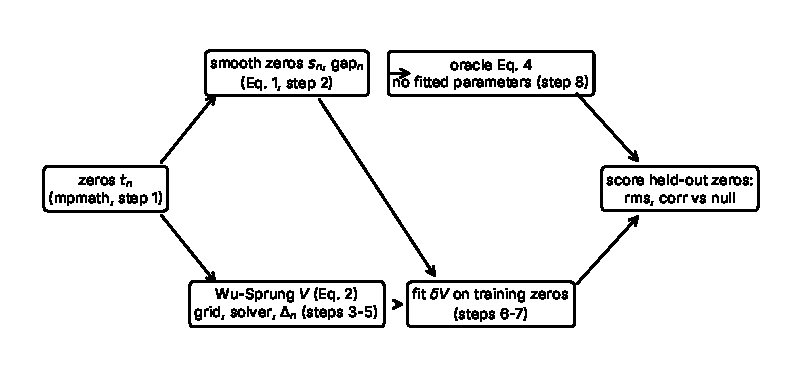
\includegraphics[width=0.95\linewidth]{figs/paper-setup_pipeline.pdf}
\caption{Schematic of the paper's protocol (Sec.~II~A--D, Appendix~A steps 1--8). Zeros and the smooth counting function feed two families of predictors: the fitted potential on the Wu--Sprung background (with bias-corrected targets) and the arithmetic oracle of Eq.~(4). Both are scored only on held-out zeros, by rms and correlation in mean spacings, against the null of their own smooth part.}\label{fig:paper-setup-pipeline}
\end{figure}

\begin{pitfall}
Do not treat ``produced with AI assistance'' as evidence for or against any number in the paper. The relevant questions are the ones you would ask of any computational work: is the pipeline archived, are seeds and versions recorded, has it been rerun independently, and do the anchors reproduce?
\end{pitfall}

\begin{keyideas}
\item Sec.~II~F discloses substantial use of Claude Fable 5 and 5.1 for code, analysis and drafting; the author reviewed all content and takes responsibility.
\item The paper commits to deterministic or seeded regeneration of every number from the archived pipeline, rerun from scratch and on a separate system.
\item Reproducibility records, not authorship tools, determine whether a numerical claim can be checked.
\end{keyideas}

\section{Paper connection}\label{sec:paper-setup-paper}
% DYK-BEGIN
\begin{didyouknow}{Trillions of Zeros Checked}
In 2021 David Platt and Timothy Trudgian published a rigorous verification that all zeta zeros with imaginary part up to $3\times10^{12}$ lie on the critical line, more than $10^{13}$ zeros in all. They used interval arithmetic to control every rounding error. Verified computations like this, together with Odlyzko's high-altitude tables, provide the kind of data such studies rely on.
\end{didyouknow}
% DYK-END

This whole chapter is a reading of the paper, so this section serves as a map. \Cref{tab:paper-setup-map} lists each part of the paper covered here, where we read it, and which earlier chapters supply its tools. Use it when you reread the paper with this chapter beside you.

\begin{table}[htbp]\centering
\caption{Map from the front half of the paper (R1 numbering) to the sections of this chapter and the tool chapters.}\label{tab:paper-setup-map}
\small
\begin{tabular}{p{0.32\linewidth}p{0.22\linewidth}p{0.36\linewidth}}
\toprule
paper element & read in & tools from \\
\midrule
Abstract & \cref{sec:paper-setup-abstract} & all of Parts I--V \\
Sec.~I, scope statement, Fig.~1 & \cref{sec:paper-setup-question} & Chs.~\ref{ch:intro}, \ref{ch:generalization}, \ref{ch:hilbert-polya} \\
Sec.~I~A (a)--(d); App.~A audit & \cref{sec:paper-setup-prior} & Chs.~\ref{ch:explicit-formula}, \ref{ch:hilbert-polya}, \ref{ch:wu-sprung} \\
Sec.~II~A, Eq.~(1), Fig.~2; App.~A steps 1--2 & \cref{sec:paper-setup-data} & Chs.~\ref{ch:asymptotics}, \ref{ch:counting-zeros}, \ref{ch:level-statistics} \\
Sec.~II~B, Eq.~(2); App.~A steps 3--5 & \cref{sec:paper-setup-solver} & Chs.~\ref{ch:wkb}, \ref{ch:wu-sprung}, \ref{ch:finite-differences} \\
Sec.~II~C (fit, other bases, OOS, within-height); App.~A steps 6--7 & \cref{sec:paper-setup-protocol} & Chs.~\ref{ch:least-squares}, \ref{ch:perturbation}, \ref{ch:fitting}, \ref{ch:generalization} \\
Sec.~II~C ``No leakage'', Eq.~(3); two nulls & \cref{sec:paper-setup-nulls} & Chs.~\ref{ch:linear-algebra}, \ref{ch:probability}, \ref{ch:finite-differences} \\
Sec.~II~D, Eq.~(4), controls A--C2; App.~A step 8; Table~V entries & \cref{sec:paper-setup-oracle} & Chs.~\ref{ch:fourier-transform}, \ref{ch:explicit-formula}, \ref{ch:sparse-frequency} \\
Sec.~II~F; Data Availability; App.~A record & \cref{sec:paper-setup-ai} & Chs.~\ref{ch:controls}, \ref{ch:paper-critique} \\
\bottomrule
\end{tabular}
\end{table}

What this chapter has \emph{not} done is interpret the results: Tables~I--III and Figs.~3--4 are read in Chapter~\ref{ch:paper-memorization}; Tables~IV--V and Sec.~IV in Chapter~\ref{ch:paper-arithmetic}; Sec.~II~E, Sec.~V and Fig.~5 in Chapter~\ref{ch:paper-spurious-floor}; Sec.~VI in Chapter~\ref{ch:paper-critique}. The numbers we did reproduce here (the nulls of Appendix~A's anchors, 0.2438, 0.2631 and 0.2739, to within a few thousandths, the scale lengths 44.883 and 59.957 of Sec.~II~B, and the Table~V entries $0.198/{+0.66}$ and $0.074/{+0.96}$) confirm that you and the paper are measuring the same things in the same units.

\section{Summary}\label{sec:paper-setup-summary}

\begin{itemize}
\item The paper tests whether potentials fitted to zeros $1,\dots,n_{\rm fit}$ predict held-out zeros; its scope is fluctuation potentials on the Wu--Sprung background in three bases, and it makes no claim against analytic constructions (\cref{sec:paper-setup-question}).
\item ``Capture'' is operational: held-out rms and correlation relative to the model's own smooth baseline; novelty is claimed only for the controlled comparison and protocol.
\item Prior work falls into four strands; the claimed gap (no held-out test of inverse-spectral fits) rests on a reproducible but bounded citation-graph keyword audit (\cref{tab:paper-setup-strands}).
\item Smooth part: $\Nsm$ of eq.~\eqref{eq:paper-setup-nsm}, smooth zeros \eqref{eq:paper-setup-sn} with closed form \eqref{eq:paper-setup-lambert}, mean spacing \eqref{eq:paper-setup-gap}, fluctuations \eqref{eq:paper-setup-fluct}; the counting residual $y_n\approx-f_n$, eq.~\eqref{eq:paper-setup-ynfn}.
\item The Wu--Sprung potential \eqref{eq:paper-setup-ws}, stably evaluated with \eqref{eq:paper-setup-wsstable}, gives $L=44.883$ and $59.957$.
\item Bias-corrected targets $\tilde t_n=t_n+\Delta_n$, eqs.~\eqref{eq:paper-setup-delta}--\eqref{eq:paper-setup-target}, remove finite-difference dispersion; Richardson uses the finer grid of a doubling pair.
\item Scoring: rms and correlation of predicted versus true fluctuations, eq.~\eqref{eq:paper-setup-score}; the null rms is the rms of the true fluctuations, eq.~\eqref{eq:paper-setup-null}.
\item The operator null is $t_n-E^{\rm Rich}_n$, eq.~\eqref{eq:paper-setup-opnull}, within $0.063$ of the smooth-zero null by \eqref{eq:paper-setup-rmsbound}; both are 0.2631 on zeros 401--500.
\item No leakage: Eq.~(3) (our \eqref{eq:paper-setup-leak}) plus the fact that $\Delta_n$ contains no zero.
\item The oracle, Eq.~(4) (our \eqref{eq:paper-setup-oracle}), has zero fitted parameters; on zeros 401--500 it gives $0.198/{+0.66}$ with one prime and $0.074/{+0.96}$ with six.
\item The controls A, B, C1, C2 are fitted on $y_n$ with hyperparameters chosen inside the training window.
\item AI assistance is disclosed; reproducibility rests on the archived, rerun pipeline and its anchors.
\end{itemize}

\section{Problems}\label{sec:paper-setup-problems}

\begin{problemlist}
\prob{1}{List the four strands of prior work in paper Sec.~I~A. For each, state whether its models (i) involve an operator, (ii) have parameters fitted to computed zeros, and (iii) according to the paper, have been evaluated on held-out zeros.}

\prob{1}{Evaluate $\Nsm(100)$ from Eq.~(1). How many zeros actually lie in $0<t\le100$? (Use \texttt{qmnt.zeros(40)} or the fact that $t_{29}<100<t_{30}$.)}

\prob{1}{Compute the local mean spacing at height $t=100$ from \eqref{eq:paper-setup-gap}.}

\prob{1}{Show directly from Eq.~(2) that $x(V_0)=0$, and explain why Eq.~(2) defines $V$ only for $x\ge0$ even though the paper's potential lives on $[-L,L]$.}

\prob{2}{For $V\gg V_0$, use $\sqrt{V-V_0}\approx\sqrt V$ in Eq.~(2) and the stable form \eqref{eq:paper-setup-wsstable} to show $x(V)\approx\frac{\sqrt V}{\pi}\log\frac{2V}{\pi e^2}$. Evaluate this at $V=1000$ and compare with $L=44.883$.}

\prob{2}{Using \texttt{scipy.special.lambertw} and \eqref{eq:paper-setup-lambert}, compute $s_{500}$ and the fluctuation $f_{500}$ of $t_{500}=811.1843588465$. Compare $s_{500}$ with \texttt{qmnt.smooth\_zeros}.}

\prob{2}{Suppose that, instead of \eqref{eq:paper-setup-delta}, the bias correction had been defined as $\Delta'_n=E^{\rm g}_n[\text{smooth}]-t_n$ for all $n$. Does the identity Eq.~(3) still hold with $\Delta'_n$? Is there now leakage? What does this tell you about the logical structure of the paper's no-leakage argument?}

\prob{2}{Using the exact discrete eigenvalues of the empty box, $E_k^{\rm disc}=\frac4{h^2}\sin^2\frac{k\pi}{2(N+1)}$, with $L=44.883$, compute the error of level $k=100$ for $N=1000$, and the error of the Richardson extrapolant built from $N=1000$ and $N=2001$ (which halves $h$ exactly). Optionally confirm with \texttt{qmnt.fd\_levels}.}

\prob{1}{Why does Table~V have a ``null'' column with rms values but no correlations for the null?}

\prob{2}{Using qmnt, compute the smooth-zero null rms on the holdouts 401--500, 501--1000 and 1001--2000, and compare with the null column of Table~V.}

\prob{2}{Using \texttt{qmnt.oracle\_zeros} and \texttt{qmnt.score}, reproduce the $\{2\}$ and 3-prime entries of Table~V for the holdout 501--1000.}

\prob{2}{With \texttt{rng = np.random.default\_rng(1)} and \texttt{test = rng.choice(400, 80, replace=False) + 1}, form a within-height random test set inside zeros 1--400. Compute the smooth-zero null on it and compare with the null range in Table~III. How many training levels does the split have?}

\prob{2}{Compute the smooth-zero null rms over the even-indexed zeros $2,4,\dots,400$ and over the odd-indexed zeros $1,3,\dots,399$. Match them to the ``odd'' and ``even'' rows of Table~III, recalling that ``odd'' means trained on odd-indexed zeros and scored on even-indexed ones.}

\prob{1}{In the interpolation split of Sec.~III, how many zeros are in the training set and how many are held out? Is it a forward, within-height, or neither kind of split in the sense of \cref{sec:paper-setup-protocol}?}

\prob{3}{From \eqref{eq:paper-setup-ynfn}, $y_n+f_n=-\delta_n^2/(4\pi\xi_n)$. (a) Explain why $y_n+f_n\le0$ always. (b) Estimate $y_{500}+f_{500}$ using $\delta_{500}=t_{500}-s_{500}$ from Problem~6. (c) Estimate $y_1+f_1$ using the Sample Problem ``Unfolding the first zero''. Verify both numerically.}

\prob{2}{Design an improved literature audit for the claim in Sec.~I~A~a. Name three changes that would address the limits listed in \cref{sec:paper-setup-prior}, and one limit that no audit can fully remove.}

\prob{1}{Match each of Appendix~A steps 1--8 to the section of the paper (II~A, II~B, II~C or II~D) where it is described.}

\prob{2}{Quote the paper's operational definition of ``capture'' (Sec.~I). Turn it into an explicit pass/fail criterion that uses the numbers 0.263 and 0 for the holdout 401--500, and apply it to the scale-1, $M=400$ operator row of Table~I (OOS $0.369$, corr $-0.07$) and the six-prime oracle of Table~V.}

\prob{3}{Let a model's predicted and true fluctuations be measured relative to a reference $R_n$, as in \eqref{eq:paper-setup-pq}. Show that the rms error is unchanged if $R_n$ is replaced by any other reference $R'_n$, but that the correlation can change. Illustrate with $f^{\rm ref}=(-1,1,0)$, $\hat f=(0.5,-0.5,0)$ and a reference change that adds $d=(0,0,3)$ to both.}

\prob{2}{Show that the GUE surmise \eqref{eq:paper-setup-gue} is normalized and has mean 1, using $\int_0^\infty s^2e^{-as^2}\,ds=\frac{\sqrt\pi}{4a^{3/2}}$ and $\int_0^\infty s^3e^{-as^2}\,ds=\frac1{2a^2}$.}

\prob{2}{Using \texttt{qmnt.zeros(10000)}, compute the fraction of unfolded spacings below $0.2$. Compare with the GUE value $\int_0^{0.2}p(s)\,ds$ and the Poisson value $1-e^{-0.2}$.}

\prob{2}{List what a reader can check, without access to the author, to test the commitments made in Sec.~II~F. Which of them can you check with \texttt{qmnt} in a few minutes?}

\prob{3}{Implement the oracle yourself: write $\Nfl$ from Eq.~(4), solve \eqref{eq:paper-setup-level} with \texttt{scipy.optimize.brentq} on the bracket $s_n\pm3\gap_n$ (widening it if the signs agree), and score zeros 401--500 with $P=\{2,3,5\}$. Compare with Table~V.}

\prob{2}{Explain, using turning points, why scale~1 scores only the first 500 levels although its box reaches $V=1000$. Compute $\Nsm(1000)$ and the number of smooth zeros below 1000, and compare with the 652 states the paper reports in Sec.~II~E.}

\prob{2}{Quantify the paper's statement that the zero precisions ``exceed every use below by many orders''. Take $t_{10000}$ from qmnt, estimate the absolute uncertainty of a 15-significant-digit value at that height, convert it to mean spacings, and compare with the smallest rms in Table~IV (0.018) and with the in-sample bound rms $<10^{-4}$ quoted in Sec.~III.}
\end{problemlist}

\section{Answers to selected problems}\label{sec:paper-setup-answers}

\textbf{1.} (a) Inverse-spectral fits \cite{wusprung,vanzyl,slater,jaksch}: operator yes, fitted to zeros yes, held-out test none found ``to our knowledge''. (b) Explicit formulae \cite{francaleclair,leclair,connes26}: no operator in the inverse-spectral sense, nothing fitted to zeros, so the held-out question does not arise. (c) Machine learning \cite{sdsu,henumberfields,vanishingorder,murmurations}: no operator; models are fitted to data and use train/test splits. (d) Operator proposals: operator yes, nothing fitted to zeros, so not applicable. The paper's own work combines operator, fitting and held-out testing.

\textbf{2.} $100/2\pi=15.9155$, $\log=2.76729$, so $\Nsm(100)=15.9155\times2.76729-15.9155+0.875=44.0427-15.9155+0.875=29.00$. Exactly 29 zeros lie below 100, so the smooth count is accurate to about a hundredth here.

\textbf{3.} $\gap=2\pi/\log(15.9155)=6.28319/2.76729=2.271$.

\textbf{4.} At $V=V_0$, $\sqrt{V-V_0}=0$, so the first term vanishes, and the argument of the second logarithm is $\sqrt{V_0}/\sqrt{V_0}=1$, whose log is 0. Hence $x(V_0)=0$. As $V$ increases from $V_0$, $x(V)$ increases from 0, so Eq.~(2) produces only $x\ge0$; the potential on $x<0$ is fixed by evenness, $V(-x)=V(x)$.

\textbf{5.} With $\sqrt{V-V_0}\approx\sqrt V$, the stable form gives the second log as $2\log(2\sqrt V/\sqrt{V_0})=\log(4V/V_0)$. Then $x\approx\frac{\sqrt V}{\pi}\bigl[\log\frac{V_0}{2\pi e^2}+\log\frac{4V}{V_0}\bigr]=\frac{\sqrt V}{\pi}\log\frac{4V}{2\pi e^2}=\frac{\sqrt V}{\pi}\log\frac{2V}{\pi e^2}$. At $V=1000$: $\sqrt{1000}/\pi=10.0658$, $\log(2000/(\pi e^2))=\log(86.157)=4.4562$, so $x\approx44.86$, about $0.03$ below the exact $44.883$. The neglected terms are of relative order $V_0/V\approx0.01$.

\textbf{6.} $z=(500-11/8)/e=183.43$; $s_{500}=2\pi(498.625)/W(183.43)\approx811.448$; $\gap_{500}=2\pi/\log(811.448/2\pi)=1.2926$; $f_{500}=(811.184-811.448)/1.2926\approx-0.204$.

\textbf{7.} Eq.~(3) is pure algebra, true for any $\Delta$, so it still holds. But now $\Delta'_n$ contains $t_n$ for held-out $n$, and the corrected target $\tilde t'_n=t_n+\Delta'_n=E^{\rm g}_n[\text{smooth}]$ no longer contains the zero at all, while the ``corrected prediction'' $E_n[\text{fit}]-\Delta'_n$ contains $t_n$: held-out truth has been inserted into the prediction. The lesson is that the no-leakage argument has two parts: the identity (correcting targets equals correcting predictions) and the construction of $\Delta_n$ from unperturbed eigenvalues only. The identity alone proves nothing.

\textbf{8.} For $N=1000$, $h=0.089676$, $E_{100}=12.2483$, $E^{\rm disc}_{100}=12.1481$, error $\approx-0.100$. With $N=2001$ the error is about a quarter of that, and $(4E_{h/2}-E_h)/3$ has error $\approx-8\times10^{-5}$, matching the next-order estimate $-E^3h^4/1440$. To see where this comes from, note that the angle $k\pi/(2(N+1))$ equals $x=\sqrt{E}\,h/2$ with $E=(k\pi/2L)^2$. Expanding $\sin^2x=x^2-x^4/3+2x^6/45-\dots$ gives $E^{\rm disc}=\frac4{h^2}\sin^2x=E-E^2h^2/12+E^3h^4/360-\dots$. In the Richardson combination the $h^2$ term cancels and the $h^4$ term is multiplied by $(4\cdot\tfrac1{16}-1)/3=-\tfrac14$, leaving $-E^3h^4/1440$.

\textbf{9.} The null predicts zero fluctuation for every held-out zero; a constant sequence has zero variance, so the Pearson correlation (covariance over the product of standard deviations) is undefined. The null rms is simply the rms of the true fluctuations, eq.~\eqref{eq:paper-setup-null}.

\textbf{11.} You should obtain rms $0.208$, corr $+0.64$ for $\{2\}$ and $0.127$, $+0.88$ for $\{2,3,5\}$, the 501--1000 row of Table~V.

\textbf{13.} Within $0.006$ of $0.238$ on the even-indexed zeros and within $0.006$ of $0.250$ on the odd-indexed zeros ( the paper's values are measured against the unperturbed potential's levels, which by \eqref{eq:paper-setup-rmsbound} can differ slightly). The ``odd'' row of Table~III scores the even-indexed zeros, so its null is 0.238; the ``even'' row scores the odd-indexed zeros, null 0.250, as printed.

\textbf{14.} Training: zeros 1--200 and 301--500, i.e.\ 400 zeros; held out: 201--300, 100 zeros. It is neither forward (the held-out zeros are below some training zeros) nor random within height; it is a contiguous interior gap, which probes a specific band of turning points.

\textbf{15.} (a) $\delta_n^2\ge0$ and $\xi_n>0$, so $-\delta_n^2/(4\pi\xi_n)\le0$. (b) $\delta_{500}=-0.2635$, $\delta^2=0.06944$, $4\pi\xi\approx4\pi(811.3)=10195$: $y_{500}+f_{500}\approx-6.8\times10^{-6}$. (c) $\delta_1=-0.3866$, $\delta^2=0.1495$, $4\pi\xi\approx4\pi(14.33)=180.1$: $y_1+f_1\approx-8.3\times10^{-4}$. The numerical values agree with these estimates.

\textbf{17.} Steps 1--2 (zeros, smooth zeros, gap): Sec.~II~A. Steps 3--5 (grids and potential, solver, bias-corrected targets): Sec.~II~B. Steps 6--7 (Hermitian fit, OOS scoring): Sec.~II~C. Step 8 (oracle): Sec.~II~D.

\textbf{19.} With $\hat f_n=(\hat t_n-R_n)/\gap_n$ and $f^{\rm ref}_n=(t_n-R_n)/\gap_n$, the difference $\hat f_n-f^{\rm ref}_n=(\hat t_n-t_n)/\gap_n$ does not contain $R_n$, so the rms is unchanged. Replacing $R_n$ by $R'_n$ adds the same sequence $d_n=(R_n-R'_n)/\gap_n$ to both $\hat f$ and $f^{\rm ref}$, which changes their covariance and variances, so the correlation can change. Example: $\hat f=(0.5,-0.5,0)$, $f^{\rm ref}=(-1,1,0)$ has correlation $-1$; after adding $d=(0,0,3)$, $\hat f'=(0.5,-0.5,3)$, $f^{\rm ref\prime}=(-1,1,3)$, both with mean 1; deviations $(-0.5,-1.5,2)$ and $(-2,0,2)$; covariance sum $1+0+4=5$; variance sums $6.5$ and $8$; correlation $5/\sqrt{52}=0.693$. The rms error stays $\sqrt{(1.5^2+1.5^2+0)/3}=1.225$. This is why the paper specifies its reference: correlations are meaningful only relative to a stated smooth baseline.

\textbf{21.} The GUE value is $\int_0^{0.2}p(s)\,ds\approx0.0084$ and the Poisson value is $1-e^{-0.2}=0.181$. The fraction from the first $10^4$ zeros is below $0.05$ (the check script confirms this bound), far closer to GUE than to Poisson: small spacings are strongly suppressed (level repulsion).

\textbf{23.} With the bracket $s_n\pm3\gap_n$ every root is found without widening at these heights, and the score is rms $0.116$, corr $+0.90$, matching the 3-prime entry of Table~V on 401--500. Your $\Nfl$ needs 9 terms: $p\in\{2,3,5\}$, $m=1,2,3$.

\textbf{25.} \texttt{qmnt} gives $t_{10000}\approx9877.78$, where the mean spacing is $2\pi/\log(9877.78/2\pi)\approx0.854$. Fifteen significant digits with four before the decimal point leave eleven after it, so the rounding error is at most $5\times10^{-12}$ in $t$, i.e.\ about $6\times10^{-12}$ spacings. The smallest rms in Table~IV is 0.018 spacings, about $3\times10^9$ times larger. Against the in-sample bound $10^{-4}$ of Sec.~III the ratio is about $1.7\times10^7$. ``Many orders'' therefore means at least seven orders of magnitude, and about nine for the held-out errors.
